\documentclass[a4paper]{scrbook}
\usepackage[utf8]{inputenc}
\usepackage[T1]{fontenc}
%\usepackage[english]{babel}
\usepackage[ngerman,english]{babel}
\usepackage{amsmath,amsfonts,amssymb} % Mathepakete
\usepackage{fancyhdr}
\usepackage{units}
\usepackage{graphicx}
\usepackage{placeins}
\usepackage{tikz,pgfplots}
\usepackage{tikz-qtree}
%\usepackage{pst-all}
\usepackage{overcite}
\usepackage{caption}
%\usepackage{bibgerm}
\usepackage{subfigure}
\usepackage{float}
\usepackage{dsfont} % Einheitsmatrix
\usepackage{mathrsfs} % geschwungenes H
\usepackage[figuresright]{rotating}
\usepackage{braket} % setzt Bra-Ket-Schreibweise richtig
\usepackage{lmodern,dsfont}
\usepackage{booktabs}
\usepackage{setspace}
\usepackage{slashbox} % erm?glicht diagonale Linien in Tabellen
\usepackage[toc,page]{appendix}
\usepackage[printonlyused,withpage]{acronym}
\usepackage{afterpage}
\usepackage{listings}
\usepackage{multirow}
\lstset{numbers=left, numberstyle=\tiny, numbersep=5pt, basicstyle=\footnotesize }
\makeatletter
\lst@AddToHook{TextStyle}{\let\lst@basicstyle\normalsize}
\makeatother

%Formatierung der Tabellen- und Bildunterschriften
\captionsetup[figure]{format=plain, justification=raggedright, singlelinecheck=false,
                      font=small, labelfont=bf}
\captionsetup[table]{position=top, format=plain, justification=raggedright,
                     singlelinecheck=false, font=small, labelfont=bf}

%pgf Bibliotheken
\usetikzlibrary{patterns,shadows,trees}
\usepgfplotslibrary{units}

% pgfplots Legenden außerhalb von Plots
\newenvironment{customlegend}[1][]{%
    \begingroup
    \csname pgfplots@init@cleared@structures\endcsname
    \pgfplotsset{#1}%
}{%
    \csname pgfplots@createlegend\endcsname
    \endgroup
}%
\def\addlegendimage{\csname pgfplots@addlegendimage\endcsname}

\newcommand{\addlegendimageintext}[1]{%
    \tikz {
        \begin{customlegend}[
            legend entries={\empty},
            legend cell align=left,
            legend style={
                draw=none,
                inner sep=0pt,
                column sep=0pt,
                nodes={inner sep=0pt}}]
        \addlegendimage{#1}
        \end{customlegend}
    }%
}


%Seitenformatierung
%\renewcommand{\baselinestretch}{1.5}
\setstretch{1.2}
%\setlength{\extrarowheight}{2pt}
\parindent = 0mm
\pagestyle{fancy}
\rhead[\leftmark]{\thepage}
\lhead[\thepage]{\rightmark}
\chead{}
\rfoot{}
\lfoot{}
\cfoot{}
\renewcommand{\headrulewidth}{0.4pt}

%%meine Farben
%\newrgbcolor{diplom1}{0.0 0.4 1.0}
%\newrgbcolor{diplom2}{0.0 0.0 0.6}
\definecolor{diplom1}{rgb}{0.0 0.4 1.0}
\definecolor{diplom2}{rgb}{0.0 0.0 0.6}
\definecolor{diplom3}{RGB}{153,0,0} %unirot
\definecolor{diplom4}{RGB}{255,165,0}
\definecolor{diplom5}{RGB}{51,37,60}

\definecolor{unirot}{RGB}{153,0,0}
\definecolor{unirot_hell}{RGB}{255,228,225}
\definecolor{lightblue}{RGB}{242.2,249.88,255}

\pgfplotsset{colormap={diplom2s}{
       color(0cm)=(white);
       color(1cm)=(diplom1);
       color(2cm)=(diplom2)}}

\pgfplotsset{compat=1.8}

\begin{document}

\setcounter{page}{1}
\thispagestyle{empty}
\tableofcontents



\begin{acronym}
  \acro{ETMD}{Electron Transfer Mediated Decay}
  \acro{ICD}{Interatomic Coulombic Decay}
  \acro{RICD}{Resonant Interatomic Coulombic Decay}
  \acro{ETI}{Excitation Transfer Ionization}
  \acro{fcc}{face-centered-cubic}
  \acro{SIP}{Single Ionization Potential}
  \acro{DIP}{Double Ionization Potential}
  \acro{HARDRoC}{Hunting Asymptotic Relativistic Decay Rates of Clusters}
  \acro{PES}{Photo-Electron Spectroscopy}
  \acro{AES}{Auger Electron Spectroscopy}
  \acro{RAS}{Resonant Auger Electron Spectroscopy}
  \acro{XAS}{X-ray Absorption Spectroscopy}
  \acro{XPS}{X-ray Photo-Electron Spectroscopy}
  \acro{NEXAFS}{Near Edge X-ray Absorption Fine Structure}
  \acro{XES}{X-ray Emission Spectroscopy}
  \acro{UPS}{Ultra-Violet Photo-Electron Spectroscopy}
  \acro{KER}{Kinetic Energy Release}
  \acro{ISR}{Intermediate State Representation}
  \acro{CES}{Correlated Excited State}
  \acro{CI}{Configuration Interaction}
  \acro{KBJ}{Kaufmann-Baumeister-Jungen}
  \acro{MCDF}{Multi-Configurational Dirac-Fock}
  \acro{SCK}{Super-Coster-Kronig}
  \acro{hcp}{hexagonal-closest-packing}
  \acro{ADC}{Algebraic Diagrammatic Construction}
  \acro{QED}{Quantum Electrodynamics}
  \acro{SCF}{Self-Consistent Field}
  \acro{CK}{Coster-Kronig}
  \acro{SCK}{Super-Coster-Kronig}
  \acro{FWHM}{Full Width Half Maximum}
%  \acro{}{}
%  \acro{}{}
%  \acro{}{}
\end{acronym}

%  \acro{}{}

 
\chapter{Introduction}
\ac{ICD} and \ac{ICD}-like processes are electronic decay processes,
which include neighbouring atoms or molecules \cite{Cederbaum97}.
They can occur after inner-valence ionization and
are most generally described by:

\begin{equation*}
 AB \quad \xrightarrow{h\nu}\quad AB^+ + e^-_{ph} \quad
    \rightarrow \quad A^+ + B^+ + e^-_{ph} + e^-_{sec}
\end{equation*}
Here, a system $AB$ is ionized in the inner-valence and the corresponding
photo-electron is emitted. The ionized system can then electronically
rearrange and as a consequence the system is split into two positively
charged components and a second electron, also called ICD electron, which is
emitted.

This kind of processes occurs in a multitude of system like noble gas clusters
and hydrogen-bonded systems. Furthermore, it has been found to explain
the electron detachment essential in repair of DNA lesions in the
photolyases enzymes \cite{Harbach13}. Furthermore, it is discussed as
source for low kinetic energy electrons in the body after an initiation
by a radioactive decay in the medical treatment of cancer. These low kinetic
energy electron cause
double strand breaks of DNA more efficiently than electrons of higher energies.
None of the competing processes has until now been proven to create these slow
electrons and to explain the locally observed damage \cite{}.

In order to be observable, two criteria, the energy and the coupling criterion,
have to be fulfilled. The energy criterion requires the energy conservation
and therefore, that the energy of the doubly ionized final state is lower than
the energy of the singly ionized initial state. If this is not the case, the
channel at hand is closed and the corresponding fragments of the
channel are not observed after the decay.
The coupling criterion requires the process to be efficient enough to compete
with other decay processes like the Auger decay (an other autoionization
process) and the radiative decay.
Hence, the study of the \ac{ICD}-like processes consists of two parts:
\begin{itemize}
 \item determination of the kinetic energy of the secondary electron
       and hence, which channels are open
 \item calculation of the decay width $\Gamma=\frac{\hbar}{\tau}$, which
       is proportional to the decay rate $\frac{1}{\tau}$ and
       anti-proportional to the lifetime $\tau$
\end{itemize}

Throughout the last decade, such processes have been studied intensively
in experiment 
and in theory using non-relativistic quantum chemistry
(see ref. \cite{Hergenhahn11} and references herein).
However, if heavy elements are involved in these decay processes, relativistic
effects might play an important role. Therefore, the aim of this
thesis is to investigate, how spin-orbit coupling and scalar-relativistic
effects influence both the energies of the involved initial and final states
as well as the decay widths of the processes.
It is going to be shown that the spin-orbit coupling leads to a larger number
of decay channels compared to the non-relativistic description. These channels
might open at different geometries of the system under investigation and
can therefore lead to channel openings at geometries, at which the channel
in the corresponding non-relativistic description would be closed. Additionally,
scalar-relativistic effects shift the energies of the initial and final states.
These shifts are most pronounced in the core region and hence might only play
a minor role for decay processes in the valence. Furthermore, the
quantity of interest is the energy difference between the initial and final
states. If the
energy shift occurs in the same direction, the effect on the measured kinetic
energy of the secondary electron is rather small.

For the calculation of the decay widths, it has to be noted that the type of
wavefunctions is inherently different than those of non-relativistic ones. They
are characterized by the total angular momentum $J$ and its projection $M_J$ rather
than the angular momentum quantum numbers $L,M_L$ and spin quantum numbers
$S,M_S$. Their spatial difference to the non-realtivistic wavefunction allows
for decays, which are non-relativistically forbidden by symmetry. E.g., the
transition between a d$_{3/2}$ and an s$_{1/2}$ state is allowed in the
relativistic description, while it breaks the Laporte rule in the non-relativistic
framework.

Non-relativistically, the decay width has been studied using asymptotic
approximations \cite{Gokhberg10_1} and various quantum chemical methods.
The asymptotic expressions for the decay width of the \ac{ICD} and a competing
\ac{ICD}-like process, the ETMD3 (Electron Transfer Mediated Decay with three
involved units), are derived in this thesis. The basic influence of
spin-orbit coupling on the decay widths of the \ac{ICD} and ETMD3 is studied
for various geometries and initial and final state symmetries.
The quantum chemical methods, which have been used for the non-relativistic 
description of the decay widths are the Wigner-Weisskopf theory \cite{Santra02},
CAP-CI
(Complex Absorbing Potential based on a Configuration Interaction wavefunction)
\cite{SakuraiModern94,Santra01_3} and FanoADC-Stieltjes \cite{Averbukh05}.
While the CAP-CI method is the most precise of the three method of the above,
it at the same
is not size-consistent and requires a huge basis set. Therefore, it is not
suited for the investigation of larger systems. In contrast to this, the
Wigner-Weisskopf theory is based on the lowest non-vanishing order of perturbation
theory and therefore computationally cheap. However, the price for this low
computational cost is the poor accuracy of the results. A compromise between
accuray and computational cost is the FanoADC-Stieltjes approach, which includes
higher perturbational orders and is size-consistent.
Therefore, the FanoADC-Stieltjes method was implemented in the relativistic
quantum chemical programme package Dirac \cite{DIRAC13} and the first results
obtained with this method are to be found in this thesis.

For the experimental validation of the \ac{ICD}-like processes, most often
noble gas clusters of 100--2000 atoms are studied. In order to compare the
theoretically obtained results with the experimental measurements, it has
to be noted that the cluster environment also affects the secondary electron
spectrum. By stabilization of ionized atoms both in the initial and final
states, the kinetic energy spectrum of the secondary electrons is shifted to
larger energies. Hence, additional channel openings might be observed.
Furthermore, the larger number of decay partners increases the decay rate
and for statistic reasons the decay rate for a specific initially ionized
atom in a heteronuclear cluster strongly depends on its position in the cluster.

In order to model the secondary electron spectra of clusters, a method
was developed based on the decomposition of cluster structures into manifolds
of decaying pairs and triples. For these pairs and triples, the kinetic energies
of the secondary electrons and the corresponding decay widths are evaluated based
on either the asymptotic expressions for the decay widths or quantum chemical
calculations for dimers and trimers. For the automatic evaluation of
a large number of cluster structures the programme
\ac{HARDRoC} \cite{HARDRoC} was developed.

The thesis is outlined as follows:

First, basic theory involved in this thesis is discussed. Afterwards, the
\emph{ab initio} methods developed and used are introduced and
finally, the obtained results are presented.
An additional description of the programmes developed in this thesis are to
be found in the appendix.

In the theory part, the large variety of autoionization processes,
especially the \ac{ICD}-like processes, is presented. Then, an introduction
into relativistic quantum chemistry and resonances, which are needed for
the calculation of the decay widths, is given. From the latter, asymptotic
approximations of the decay width for the \ac{ICD} and ETMD3 are derived
in the relativistic framework.
Finally, noble gas clusters and their experimental creation and measurement
are presented.

In the method part, the description of continuum properties with $\mathcal{L}^2$
functions, the \ac{ADC} and especially the FanoADC-Stieltjes approach are
presented.

In the results part, the systems are studied with increasing number of constituents.
First, Auger processes of noble gas atoms are studied for testing purposes
of the relativistic FanoADC-Stieltjes implementation and in order to investigate
basic relativistic effects. Then, channel openings and decay widths for
different geometries of pairs and triples are studied including relativistic
effects. Afterwards, the relative asymptotic decay width behaviour
of different decay channels, which are split due to spin-orbit coupling are
investigated. After this, the decay widths of the ArXe dimer is investigated
using the relativistic FanoADC-Stieltjes approach. Finally, secondary electron
spectra of heteronuclear ArXe and NeAr clusters are studied based on the
results of the preceding chapters.
In the ArXe clusters, relativistic effects, basic effects of the cluster environment
and different cluster structures are investigated.
For the NeAr clusters, a new procedure to determine structural information of mixed
noble gas clusters with competing \ac{ICD} processes is presented.

\chapter{Theory}

\section{Autoionization Processes}
\section{Clusters}
\section{Relativistic Quantum Chemistry}
 \section{Resonances}

Classically, a resonance is the maximum coupling of two or more
oscillating systems, in which energy is either transferred from 
one system to another or converted into a different kind of energy.
In quantum mechanics analogously the maximum coupling of an initial 
state to either 
another state or to
a continuum of states is referred to as a resonance. Hereby this
interaction can be mediated via an external field.
In consequence of the coupling the system evolves over time from
the initial state into at least one other state. Depending on the investigated
process, this change is either reversible like in Rabi oscillations \cite{Rabi}
or irreversible like in our case of autoionization processes.

The time evolution of a resonance process can be characterized by
the averaged lifetime $\tau$ of the initial state or its counterpart
in the energy domain,
the averaged decay width $\Gamma = \frac{\hbar}{\tau}$.

Historically the underlying theory was developed by numerous scienctists
like Dirac \cite{Dirac27_1,Dirac27_2}, Wentzel \cite{Wentzel27}, 
Weisskopf and Wigner \cite{Weisskopf30},
Fermi \cite{Fermi32}, Breit and Wigner \cite{Breit36},
Kapur and Peierls \cite{Kapur38}, Siegert \cite{Siegert39} and many others.

In the following we are going to discuss the necessary basics of scattering
theory as summarized by Gell-Mann \cite{Gell-Mann53}.


%Its time evolution and optionally the corresponding decay width has historically
%been investigated using either perturbation \cite{} or scattering
%theory \cite{} until it became part of Feshbach's unified theory of
%nuclear reactions \cite{Feshbach58,Feshbach62}. This completely general theory
%is based on projection operators partitioning the Hilbert space into subspaces of
%initial and final states.
%In contrast to earlier approaches, it holds for all coupling schemes as well as
%all quantum numbers. They will be taken care of in the definition of the
%projection operators.
%Shortly after,
%Fano amplified the latter ansatz to describe excitation spectra, which
%are inverse processes to Feshbach's nuclear reactions.\cite{Fano61}


We start from the time dependent Schroedinger equation

\begin{equation}
  i \frac{\mathrm{d}}{\mathrm{d}t} \Psi(t) = (K + V) \Psi(t) ,
\end{equation}
where $K$ denotes the Hamilton operator of non-interacting colliding
particles, or in our case initial and final states. Its solution
$\Phi_i(t) = \phi_i e^{-iE_it}$ are stationary states of the system.

\begin{equation}
  i \frac{\mathrm{d}}{\mathrm{d}t} \Phi(t) = K \Phi(t)
\end{equation}

Out purpose it the description of the transition rates from an initial state
$\Phi_i(t)$ to a final state $\Phi_f(t)$ mediated by the interaction $V$ between
them. We are going to achieve this by taking the time derivative of the system's
probability $\omega_{fi}(t)$ to be in a certain final state at time t.

\begin{align}
  w_{fi}(t) &= \frac 1{N_i} |f_{fi}|^2 \\
  f_{fi}(t) &= \braket{\Phi_f(t)|\Psi_i(t)} \label{equation:scattering_overlap}\\
  N_i       &= \braket{\Psi_i(t)|\Psi_i(t)}
\end{align}

In eq. (\ref{equation:scattering_overlap}) not the stationary state $\Phi_i$
has been chosen to represent the initial state but $\Psi_i$. Since our knowledge
about the initial state wave function is limited to its behaviour without the
interaction $V$, being turned on at $t=0$, we have to describe the initial state
wave function at some time in the distant past $T<0$ and propagate it until $t=0$.
Therefore the question arises, which time $T$ should be selected for this purpose.
Since no time is better than any other and the result might depend on the decision,
one averages over propagations starting at different times $T$.

\begin{equation}
  \Psi_i(t) = \frac 1\tau \int\limits_{-\tau}^0 \mathrm{d}T \,
              e^{-iH(t-T)} \, \Phi_i(T)
\end{equation}
Here $\tau$ is allowed to approach $+\infty$ at the end of the calculation.

A more convenient way to include this ansatz in the further derivation
is its Fourier transformation
\begin{equation}
  \Psi_i(t) = \varepsilon \int\limits_{-\infty}^0 \mathrm{d}T \,
              e^{\varepsilon T} e^{-iH(t-T)} \Phi_i(T)
\end{equation}

with $\varepsilon = \tau^{-1}$. Evaluating the integral, this leads to:
\begin{align}
   \Psi_i(t) &= \varepsilon \, e^{-iHt} \int\limits_{-\infty}^0 \mathrm{d}T \,
                e^{\varepsilon T} e^{i(H-E_i)T} \phi_i\\
             &= e^{-iHt} \frac{\varepsilon}{\varepsilon+i(H-E_j)} \phi_i .
\end{align}

Using the Schroedinger equation
\begin{equation}
  (H-E_i) \phi_i = V \phi_i
\end{equation}

of the whole system, one easily arrives at an expression for the initial state
at time $t=0$.
\begin{align}
  \Psi_i(0) &= \frac{\varepsilon + i(H-E_i) - i(H-E_i)}{\varepsilon + i(H-E_i)} \phi_i\\
            &= \phi_i + \frac{1}{E_i-H+i\varepsilon} V \phi_i \label{equation:in_state_0}\\
            &\approx \phi_i + \frac{1}{E_i-K+i\varepsilon} V \Psi_i(0) \label{equation:in_state_0_approx}
\end{align}

The latter equation holds for a small perturbation $V$ as can be seen by comparing
the power expansions of equations (\ref{equation:in_state_0}) and
(\ref{equation:in_state_0_approx}).\\
Since the norm $N_{fi}$ is time-independent, we now have
everything we need for the determination of the decay rate.
Inserting equation (\ref{equation:in_state_0_approx}) into equation
(\ref{equation:scattering_overlap}) we evaluate the overlap between the initial
and the final state.
\begin{equation}
  f_{fi}(0) = \delta_{fi} + \frac{1}{E_i-E_f+i\varepsilon} R_{fi}(\varepsilon)
\end{equation}

Here, 
\begin{equation}
  R_{fi}(\varepsilon) = \braket{\phi_f|V|\Psi_i(0)}
\end{equation}
denotes the coupling of the initial with the final state via the interaction
operator $V$.

The time dependence of coupling between the two time-independent states is now
introduced to give:
\begin{equation}
  f_{fi}(t) = \braket{\phi_f| e^{i(E_f-H)t} |\Psi_i(0)} .
\end{equation}

Its absolute square is proportional to the probability of the system to be
in the final state $\phi_f$ and its time derivative at $t=0$ yields
\begin{equation}
  \left . \frac{\mathrm{d}}{\mathrm{d}t} |f_{fi}|^2 \right |_{t=0}
  = 2\delta_{fi} \operatorname{Im}R_{ii}(\varepsilon) 
    + \frac{2\varepsilon}{(E_i-E_f)^2+\varepsilon^2} |R_{fi}(\varepsilon)|^2 .
\end{equation}

It consists of two parts, the first is propotional to the probability to stay
in the initial state and the second one describes the transition into the
final state. The latter has the typical Lorentzian shape with the full width
half maximum
(FWHM) $2 \varepsilon$ (further information can be found in the appendix
\ref{section:app_cauchy}). From now on
the full width half maximum ${2\varepsilon}$ will be called the
decay width $\Gamma$.
The larger the width is, the faster is the transition into the final state.

%\begin{figure}[h]
%  \centering
%  % \begin{tikzpicture}[
          scale=1.0,>=stealth,domain=0.5:10,samples=100,
          declare function={
          gamma = 1.0;
          factor = 16.0;
          halfmax = factor * 0.15915;
          x_0 = 5.0;
          distrib(\x) = factor/3.14159 * gamma / ((\x-x_0)^2 + gamma^2);
        }]
%     \tiny
%  \draw[very thin,color=gray] (-0.1,-0.1) grid (4.9,4.9);
  \draw[->,thick] (-0.2,0) -- (10.2,0) node[right] {$x$};
  \draw[->,thick] (0,-0.2) -- (0,7.2) node[above] {$f(x,x_0,\gamma)$};
  % add ticks
  \draw [thick] (5,0) -- (5,-5pt) node [anchor=north] {$x_0$};

  \draw [color=black,domain=0:10,smooth,very thick]    plot
         (\x,{distrib(\x)});% node [anchor=south] {Cauchy distribution};
  \draw [-,very thick,diplom1] (4.0,halfmax) -- (6,halfmax)
         node [anchor=south west] {$2\gamma$};
 \end{tikzpicture}

%%  \caption{}
%  %\label{figure:cauchy-dist}
%\end{figure}




\subsection{Resonances in systems with more than two states}

In the case of a multistate system, the calculation of the decay width is more
complex than in a system with only two states.
This difficulty is overcome by partitioning the Hilbert space into initial and final
state subspaces and using the approriate eigenfunctions of these subspaces for the
calculation of the decay widths. 
Several theories had been used for the description of different nuclear reactions
before they were first unified by Feshbach in 1958 \cite{Feshbach58,Feshbach62,Feshbach_book}.
In contrast to earlier approaches, it holds for all coupling schemes as well as
all quantum numbers. They will be taken care of in the definition of the
projection operators.
Shortly after,
Fano amplified the latter ansatz to describe excitation spectra, which
are inverse processes to Feshbach's nuclear reactions.\cite{Fano61}

It has to be noted, that the applied criteria for the seletion of
these subspaces affect the final results.

Starting from the Schroedinger equation of the total system under investigation

\begin{equation}
  H \Psi = E \Psi \label{schroedinger}
\end{equation}

the projection operators $P$ and $Q$ are defined. $P$ projects the final state out
of the total wavefunction $\Psi$ and is defined with respect to eigenstates
of the system in the asymptotic time limit, which means long after the process
itself finished. $Q$ is analogously defined with respect to the rest of the
system as $Q = 1 - P$. Therefore after insertion to eq. \ref{schroedinger}

\begin{equation}
  H (P+Q) \Psi = E \Psi
\end{equation}

\begin{align}
  (E - H_{PP}) P \Psi & = H_{PQ} Q \Psi \label{se_PP}\\
  (E - H_{QQ}) Q \Psi & = H_{QP} P \Psi \label{se_QQ}
\end{align}

can easily be derived with

\begin{align*}
  H_{PP} & \equiv PHP & \quad\quad H_{PQ} & \equiv PHQ\\
  H_{QP} & \equiv QHP & \quad\quad H_{QQ} & \equiv QHQ .
\end{align*}

From equation \ref{se_QQ} a straigth-forward solution for the system excluding
the selected final states can be found.

\begin{equation}
  Q \Psi = \frac{1}{E^{(+)}-H_{QQ}} H_{QP} P \Psi \label{feshbach_qpsi}
\end{equation}

The latter expression holds in case of selectively chosen open channels, which
do not represent all open channels. In case of all open channels being selected,
$E^{(+)}$ is to be substituted by $E$.

After insertion of eq. \ref{feshbach_qpsi} into eq. \ref{se_PP} one arrives at

\begin{equation}
  \mathscr{H} \,P \Psi = E \,P \Psi \label{se_ppsi}
\end{equation}

with $\mathscr{H}$ being the effective Hamiltonian of the final states.
\begin{equation}
  \mathscr{H} = H_{PP} + H_{PQ} \frac{1}{E^{(+)}-H_{QQ}} H_{QP}
\end{equation}

In order to solve these expressions we define $\{\Phi_n\}$ to be the solutions
of the Hamiltonian excluding the final state solutions or the closed channels
solutions in case of all open channels being defined as final states.
They are assumed to be bound and to fulfill the
Schroedinger equation

\begin{equation}
  (\varepsilon_n - H_{QQ}) \Phi_n = 0 .
\end{equation}

This approach is not exact, because the states being bound implicate
their lifetimes to be infinite, which they are intrinsically
to the problem not supposed to be. However, for states having a long lifetime,
this approximation is reasonable. -> How long is long?

Together with a set of continuum wavefunctions $\{\Phi(\alpha,E)\}$, they are
defined to fulfill the following orthogonality relations

\begin{align}
  \braket{\Phi_n|\Phi_n} = 1 \quad  & \quad \braket{\Phi_n|\Phi(\alpha,E)} = 0\\
  \braket{\Phi(\alpha,E)|\Phi(\alpha',E')} & = \delta(\alpha-\alpha') \delta(E-E')
\end{align}

and to form an orthonormal basis. These continuums wavefunctions are characterized
by their energy $E$ and their quantum numbers, which are at this stage embraced
to the variable $\alpha$.

\begin{equation}
  1 = \sum\limits_n \ket{\Phi_n}\bra{\Phi_n} + \int \mathrm{d}\alpha \int \mathrm{d}E
      \ket{\Phi(\alpha,E)}\bra{\Phi(\alpha,E)} \label{feshbach_1}
\end{equation}

Expanding eq. \ref{se_ppsi} into this complete set yields an effective Hamiltonian
of

\begin{equation}
  \mathscr{H} = H_{PP}\, + \,
  \sum\limits_n H_{PQ} \,\frac{\ket{\Phi_n}\bra{\Phi_n}}{E^{(+)}-\varepsilon_n}\, H_{QP} \,+\,
  \int \mathrm{d}\alpha \int\mathrm{d}E \,H_{PQ} \,
  \frac{\ket{\Phi(\alpha,E)}\bra{\Phi(\alpha,E)}}{E^{(+)}-\varepsilon} \, H_{QP}
\end{equation}

which is useful to split into two parts. One describing the Hamiltonian of the
initial state being in resonance with the continuum $\Phi_s$ with its energy
$\varepsilon_s$ varying strongly close to the resonance energy and the rest
$\mathscr{H}'$

\begin{equation}
  \mathscr{H} = \mathscr{H}' + H_{PQ} \,\frac{\ket{\Phi_s}\bra{\Phi_s}}{E^{(+)}-\varepsilon_s}\, H_{QP}
\end{equation}

with
\begin{equation}
  \mathscr{H}' = H_{PP}\, + \,
  \sum\limits_{n\ne s} H_{PQ} \,\frac{\ket{\Phi_n}\bra{\Phi_n}}{E^{(+)}-\varepsilon_n}
  \, H_{QP} \,+\,
  \int \mathrm{d}\alpha \int\mathrm{d}E \,H_{PQ} \,
  \frac{\ket{\Phi(\alpha,E)}\bra{\Phi(\alpha,E)}}{E^{(+)}-\varepsilon} \, H_{QP} .
\end{equation}

This reformulation leads to the following version of eq. \ref{se_ppsi}
\begin{equation}
  (E - \mathscr{H}')\, P \Psi =
   H_{PQ} \,\frac{\ket{\Phi_s}\bra{\Phi_s}}{E^{(+)}-\varepsilon_s}\, H_{QP} P \Psi = \mathscr{V} P \Psi.
\end{equation}

The eigenfunctions of $\mathscr{H}'$ have to fulfill outgoing boundary conditions,
which is labelled by the superscript $(+)$

\begin{equation}
  (E-\mathscr{H}') \psi_f^{(+)} = 0 \label{sol_outg} .
\end{equation}

This relation can the be utilized to find a solution for $\ket{p \Psi}$ analogous
to the approach in equation (\ref{equation:in_state_0_approx}):

\begin{equation}\label{sol_ppsi}
  P \Psi = \psi_f^{(+)} + \frac{1}{E^{(+)} - \mathscr{H}'}
           \frac{H_{PQ}\ket{\Phi_s}
           \braket{\Phi_s|H_{QP}|P\Psi}}{E^{(+)} - \varepsilon_s} .
\end{equation}

$\ket{P \Psi}$ still depends on itself. Therefore 
eq. \ref{solppsi}
is multiplied from the left with $\bra{\Phi_s|H_{QP}}$ to give:
\begin{equation}
  \braket{\Phi_s|H_{QP}|P\Psi} = \braket{\Phi_s|H_{QP}|\Psi_f^{(+)}} +
  \frac{1}{E^{(+)} - \mathscr{H}'}
  \frac{\braket{\Phi_s|H_{QP}H_{PQ}|\Phi_s} \braket{\Phi_s|H_{QP}|P\Psi}}
       {E^{(+)} - \varepsilon_s}  \label{s_ppsi} .
\end {equation}

Defining the quantity

\begin{equation}
  W_{QQ} = H_{QP}\frac{1}{E^{(+)} - \mathscr{H}'}H_{PQ}
\end{equation}

and solving eq. \ref{s_ppsi} for

\begin{equation}
  \braket{\Phi_s|H_{QP}|P\Psi} = \frac{\braket{\Phi_s|H_{QP}|\Psi_f^{(+)}}(E-\varepsilon_s)}
{E - \varepsilon_s - \braket{\Phi_s|W_{QQ}|\Phi_s}}
\end{equation}

yields the following expression:
\begin{equation}\label{}
  P \Psi = \psi_f^{(+)} + \frac{1}{E^{(+)} - \mathscr{H}'}
           \frac{H_{PQ}\ket{\Phi_s}
           \braket{\Phi_s|H_{QP}|\psi_f^{(+)}}}
           {E^{(+)} - \varepsilon_s - \braket{\Phi_s|W_{QQ}|\Phi_s}} .
\end{equation}

It can be shown, that it is not necessary to calculate $f_{fi}$, but that the
so-called transition matrix

\begin{equation}
  \mathscr{T}_{fi} = \braket{\psi_i^{(-)}|V|\phi_f},
\end{equation}

carries all the necessary information about the properties of interest as
decay widths and cross sections.
Here $\phi_f$ denotes the final states in our represented by $\ket{P \Psi}$ and
$\psi_i^{(-)}$ are incoming states with appropriate boundary conditions fulfilling

\begin{equation}
  (E - \mathscr{H}') \psi_i^{(-)} = 0 .
\end{equation}

This leads us to the following expression for the transition matrix

\begin{equation}
  \mathscr{T}_{if} = \mathscr{T}_{if}^{(P)} + 
                     \frac{\braket{\psi_i^{(-)}|H_{PQ}|\Phi_s}
                           \braket{\Phi_s|H_{QP}|\Psi_f^{(+)}}}
                          {E-\varepsilon_s - \braket{\Phi_s|W_{QQ}|\Phi_s}}
\end{equation}

where $\mathscr{T}_{if}^{(P)}$ describes the transitions without any interaction
between the initial and final states taken into account. Therefore, in the case
of thoroughly partitioning of contributions into initial and final states,
this part is supposed to be zero. The second part describes the transition
from the initial into the final states mediated by the interaction between them.

The transition matrix is from here on handled analogously to $f_{ij}$ in the preceding subsection.
An explicit time-dependency is introduced, the absolute square is differenciated
with respect to the time and evaluated for $t=0$.
The derived expression shows again a Lorentzian shape with a width proportional to
the imaginary part of $\braket{\Phi_s|W_{QQ}|\Phi_s}$. We therefore split it into
its real and imaginary part by introducing a delta function using 
$\lim\limits_{\varepsilon \to 0_+} \frac{1}{x+i\varepsilon} = \mathscr{P} \frac 1x \mp i\pi\delta(x)$,
where $\mathscr{P}$ is the principal part and $\delta(x)$ denotes the
Dirac delta function. \cite{Cohen_Tannoudji_3_2}

\begin{align}
  \braket{\Phi_s|W_{QQ}|\Phi_s} & = \Delta_s(E) - i \frac{\Gamma_s(E)}{2}\\
                                & = \braket{\Phi_s|H_{QP}
                                    \frac{1}{E^{(+)}  - \mathscr{H}'}H_{PQ}|\Phi_s}\\
                                & = \braket{\Phi_s|H_{QP}
                                    \frac{\mathcal{P}}{E - \mathscr{H}'}H_{PQ}|\Phi_s}
                                    - i\pi \braket{\Phi_s|H_{QP}\delta(E-\mathscr{H}')H_{PQ}
                                    |\Phi_s} 
\end{align}

Inserting the latter expression into the transition matrix yields

\begin{equation}
  \mathscr{T}_{if} = \mathscr{T}_{if}^{(P)} + 
                     \frac{\braket{\psi_i^{(-)}|H_{PQ}|\Phi_s}
                           \braket{\Phi_s|H_{QP}|\Psi_f^{(+)}}}
                          {E-\varepsilon_s - \Delta_s + i \frac{\Gamma}{2}}
\end{equation}

from which now the real part of $\braket{\Phi_s|W_{QQ}|\Phi_s}$ can be interpreted 
as an energy shift $\Delta_s(E)$ of the resonance introduced by the interaction of the initial
with the final states and its imaginary part to carry the information about the
decay width $\Gamma_s(E)$ and hence the lifetime.

%The complex matrix element $\braket{\Phi_s|W_{QQ}|\Phi_s}$ wears the influence
%of the coupling on the rest of the system. Its real part can be identified as
%an energy shift $\Delta_s(E)$ to the "unperturbed" resonance energy whereas its
%complex part is connected to the decay width $\Gamma_s(E)$.





From the imaginary part of $\braket{\Phi_s|W_{QQ}|\Phi_s}$ the decay width can easily be concluded. Inserting a complete set
of eigenfunctions as defined in eq. \ref{sol_outg} the decay width can be described
as a sum over the different open channel solutions for a given resonant state.
\begin{align}
  \Gamma_s & = 2 \pi \braket{\Phi_s|H_{QP}\delta(E-\mathscr{H}')H_{PQ}|\Phi_s}\\
           & = 2 \pi \sum\limits_r \left | \braket{\Phi_s|H_{QP}|\psi_r^{(+)}} \right|^2\\
           & = \sum\limits_r \Gamma_{sr}(E)
\end{align}

\section{Decay Rates}
\subsection{Decay Rates of ICD-like Processes in the Asymptotic Limit}


\chapter{Methodology}
\section{general stuff}
\section{Algebraic Diagrammatic Construction}
\section{Description of Interactions of Bound and Continuum States}
\section{Decay Width Determination by Moment Theory}
 \chapter{Obtaining Continuum Properties from $\mathcal{L}^2$-Functions}


\section{Bound and Continuum States}
Before we describe the decay of a metastable state, we have to remember,
that both bound and continuum states are involved in such a process.
Bound states are very localized and in quantum mechanics
represented by square integrable
functions of the $\mathcal{L}^2$ Hilbert space. Their boundary conditions
lead to a quantized energy spectrum and the functions of the bound states
are normalized
to represent one particle each. Unperturbed bound states are stationary
and can therefore conveniently be described using the time-independent
Schroedinger equation.
In contrast to the bound states the
continuum states are very delocalized, are not $\mathcal{L}^2$
integrable and are hence not accessible for a probabilistic interpretation.
Their energy spectrum is continuous and the functions are normalized to
their respective energy.

In decay processes
where bound and continuum states interact, it is obliged to find a way to
properly represent bound states in an energy normalization or continuum states
in an $\mathcal{L}^2$ normalization.
Since most quantum chemical programme packages are based
on $\mathcal{L}^2$ functions,
it is most convenient to go for the latter approach.
Especially for properties like decay widths or ionization cross sections, one
possibility is to interprete the evaluation of an expectation value
including the continuuum in either the initial or the final state as
Gaussian quadrature and compare them to analogous expressions for the
expectation value in a discrete set of eigenstates. The given equivalence
allows to use the machinery of Gaussian quadrature combined with an imaging
procedure, both known in the literature,
for the determination of the required entity. \cite{Reinhardt79}

After an explanation of Gaussian quadrature we are going to show how
the discrete spectrum of a Hamiltonian in $\mathcal{L}^2$ representation
can be motivated to contain information of the continuum using Gaussian quadrature
based on the discussion of \cite{Reinhardt79}.
Then we are going to show, how the decay width can be obtained from a
discrete pseudo-spectrum by using Stieltjes imaging \cite{Langhoff76,Corcoran77}.
Finally we are going to introduce the FanoADC approach for the creation of
states in the $\mathcal{L}^2$ \ac{ISR} basis.



\section{Gaussian Quadrature}
The gaussian quadrature is a numerical method for integration. By approximating
the function to be integrated $g(x) = \rho(x) f(x)$ to be a product of a
positive definite weight
function $\rho (x)$ and a continuous and bounded function $f(x)$. \cite{Wikipedia_Gauss_Quadratur}
The evaluation of the integral is then desired to be obtained as

\begin{equation}
  \int\limits_a^b \rho(x) f(x) dx \approx \sum\limits_{i=1}^n \omega_i f(x_i)  .
\end{equation}

Here the weigths $\omega_i$ and the abcissae $x_i$ are to be determined
analytically, if possible, or otherwise in an optimal way. This leads the abcissae
to be unequally spaced unlike in the basic
integration schemes using the trapezoidal rule.

The function $f(x)$ can be expressed as a polynomial.
For certain weight functions and boundaries
of integration, these
polynomials can be determined analytically.
It can furthermore be shown, that the roots (zeros) of the highest order polynomial
describing the function $f(x)$ give the optimal abcissae $x_i$.
These polynomials $Q_n$ are normalized with respect to the weight function as

\begin{equation}
  \int\limits_{-1}^{1} \rho(x) Q_n(x) Q_m(x) = N_n \delta_{nm}  ,
\end{equation}
where $N_n$ denotes the normalization factor.


In the special case of the weight function
$\omega(x)= \frac{1}{\sqrt{1-x^2}}$ and the interval $[-1,+1]$
the solution to the polynomials are the so-called Chebyshev polynomials, with
the analytical abscissae and weights

\begin{equation}
  x_{i,n} = \cos \left( \frac{2i-1}{2n} \pi \right)
  \quad\quad \omega_{i,n} = \frac \pi n .
\end{equation}

\begin{figure}[ht]
  \centering
  \begin{tikzpicture}
    \begin{axis}[%scale=0.8,
                 domain=-1.0:1.0,
                 samples = 200,
                 %xtick={-3.14159,-1.57089,...,3.14159},
                 %xticklabels={$-\pi$,$-\frac \pi 2$,0,$\frac \pi 2$,$\pi$},
                 cycle list name = exotic,
                 legend style={anchor= north west},
                 legend cell align = left
                 ]
     \addplot+[domain=-1:-0.965925826289+0.135517335117/2,
              diplom1,
              mark = none,
              %forget plot,
              pattern = north east lines,
              pattern color = diplom1
              ]
              {0.0987789349866} \closedcycle;
     \addlegendentry{approximation of the integral}
     \addplot+[domain=-0.965925826289+0.135517335117/2:-0.707106781187+0.370240244847/2,
              diplom1,
              mark = none,
              forget plot,
              pattern = north east lines,
              pattern color = diplom1
              ]
              {0.646446609407} \closedcycle;
     \addplot+[domain=-0.707106781187+0.370240244847/2:-0.258819045103+0.505757579964/2,
              diplom1,
              mark = none,
              forget plot,
              pattern = north east lines,
              pattern color = diplom1
              ]
              {0.982662411472} \closedcycle;
     \addplot+[domain=-0.258819045103+0.505757579964/2:0.258819045103+0.505757579964/2,
              diplom1,
              mark = none,
              forget plot,
              pattern = north east lines,
              pattern color = diplom1
              ]
              {1.017337588535} \closedcycle;
     \addplot+[domain=0.258819045103+0.505757579964/2:0.708718898022+0.370240244847/2,
              diplom1,
              mark = none,
              forget plot,
              pattern = north east lines,
              pattern color = diplom1
              ]
              {1.353553390592} \closedcycle;
     \addplot+[domain=0.708718898022+0.370240244847/2:1.0,
              diplom1,
              mark = none,
              forget plot,
              pattern = north east lines,
              pattern color = diplom1
              ]
              {1.901221065013} \closedcycle;
     \addplot [diplom2, thick]
              {x^3 + 1};
     \addlegendentry{$f(x)= x^3 + 1$}
     %\addplot [diplom3, thick]
     %         {x^4/4 + x};
     \addplot [only marks,mark=o,thick]
       coordinates {
                   ( 0.965925826289, 1.901221065013 )
                   ( 0.707106781187, 1.353553390592 )
                   ( 0.258819045103, 1.017337588535 )
                   (-0.258819045103, 0.982662411472 )
                   (-0.707106781187, 0.646446609407 )
                   (-0.965925826289, 0.0987789349866)
                   };
     \addlegendentry{$f_i(x_i)$}
    \end{axis}
\end{tikzpicture}

  \caption{Integration by Gauss-Chebyshev quadrature of the function
           $h(x)=x^3 + 1$ (dark blue) with $n=6$. The integral (light blue)
           is approximately obtained by summation
           over all product of optimal abcissae and weights $x_ih(x_i)$ (circles).}
  \label{figure:gaussian_quadrature}
\end{figure}

This means, that the integration of an arbitrary function $h(x)$ within
the interval $[-1,1]$ can be integrated as

\begin{equation}
  \int\limits_{-1}^1 h(x) dx = \int\limits_{-1}^1 \omega(x) \sqrt{1-x^2} h(x) dx
  \approx \frac \pi n \sum\limits_{i_1}^n h(x_i) \sqrt{1-x_i^2}
\end{equation}

An example for such an integration is shown in figure \ref{figure:gaussian_quadrature}
for $h(x) = x^3 + 1$. The dark blue curve shows $h(x)$, the points are the
calculated $h_i$ at the abcissae $x_i$ and the light blue hatched areas are the
approximations to the integral for the certain areas. Obviously, the finer the
grid for the integration is, the more precise is the the approximation to
the analytical integral going to be.

The above discussion holds for a known weight function.
For an unknown weight function, the integral can be obtained by solving the so-called
moment problem. \cite{Reinhardt79}




\section{Expressing the Continuum Properties in Terms of Gaussian Quadrature}
The Hamiltonian can be expressed in terms of a complete set of eigenfunctions

\begin{equation} \label{equation:complete_hamniltonian}
  H = \sum\limits_i \ket{\phi_i} E_i \bra{\phi_i}
     + \int\limits_0^\infty \mathrm{d}E \ket{\phi(E)} E \bra{\phi(E)}  ,
\end{equation}
where the manifold of $\phi_i$ denote the bound state eigenfunctions being orthonormal
in the sense of the probabilistic picture $\braket{\phi_j|\phi_i} = \delta_{ij}$.
The continuum functions $\phi(E)$ also form an orthonormal set of basis functions
but are normalized with respect to their energy.

\begin{equation}
  \braket{\phi(E) | \phi(E')} = \delta(E-E')
\end{equation}

In a calculation using a finite $\mathcal{L}^2$ basis, the diagonalization of the
Hamiltonian yields an approximative set of eigenfunctions $\chi_i$ with corresponding
eigenvalues $\tilde{E}_i$ such that

\begin{equation}
  \tilde{H} \ket{\chi_i} = \tilde{E}_i \ket{\chi_i} \quad\quad  \,
  \braket{\chi_j|\chi_i} = \delta_{ij} .
\end{equation}

If we now rewrite the approximative Hamiltonian in terms of these $\mathcal{L}^2$
functions, we obtain

\begin{equation}
  \tilde{H} = \sum\limits_{E_i<0} \ket{\chi_i} \tilde{E}_i \bra{\chi_i}
            + \sum\limits_{E_j>0} \ket{\chi_j} \tilde{E}_j \bra{\chi_j}   ,
\end{equation}
where the first part with eigenvalues smaller than 0 corresponds to the
bound states and the second part with energies higher than 0 corresponds to
the continuum. In this representation the continuum is not described explicitely,
but in a discretized representation.

The eigenfunctions and eigenvalues of the positive energy solutions have no physical
meaning, because for more and more complete bases, the energies will approach zero
and the eigenfunctions will be arbitrarily diffuse. Still, they inhibit a useful
mathematical meaning if the continuum part is interpreted in terms of
a numerical quadrature.
In the case of integrating the continuum part of equation
\ref{equation:complete_hamniltonian} for evaluation of the energy expectation
value $\braket{\Psi| H | \Psi}$ in the full Hamiltonian or the discretized Hamiltonian
$\braket{\Psi| \tilde{H} | \Psi}$
with first gaussian quadrature 


\begin{align}
  \int\limits_0^\infty \mathrm{d}E \braket{\Psi|\phi(E)} E \braket{\phi(E)|\Psi}
  &\simeq \sum\limits_j \omega_j \braket{\Psi|\phi(E_j)} E_j \braket{\phi(E_j)|\Psi} ,
\end{align}
where  $\omega_j$ are the quadrature weights and second the discrete positive energy
eigenfunctions, the continuum part of the expectation value reads as


\begin{equation}
  \int\limits_0^\infty \mathrm{d}E \braket{\Psi|\phi(E)} E \braket{\phi(E)|\Psi}
  \simeq \sum\limits_{E_j}  \braket{\Psi|\chi} \tilde{E}_j \braket{\chi|\Psi}   .
\end{equation}

In both cases, the integral is approximated by a sum and in some special cases, where
the analytic continuum functions are known, it can be shown from the results,
that there seems to be a one-to-one corespondence between each $\mathcal{L}^2$
eigenfunction of the positive energy part and the continuum function evaluated
at the energy $\tilde{E}_j$. The equivalent quadrature weight connects the discrete and
the continuum function for the given energy and can be interpreted as a renormalization.

\begin{equation}
  \ket{\chi_j} = \sqrt{\omega_j^{Eq}} \ket{\phi(\tilde{E}_j)}
\end{equation}

In the following, we are going to assume, that this equivalence between $\mathcal{L}^2$
and continuum functions with the integral interpreted as Gaussian quadrature
is true for all our systems under investigation.

If we for a moment assume, that we knew the appropriate equivalent quadrature
weigths, we could calculate the decay width from a continuous representation as
from equation \ref{equation:Gamma_HE}.

\begin{equation}
  \Gamma = \frac 1{\omega_{j}^{Eq}} \left| \braket{\Phi_s|\mathcal{H}'-E|\chi_j} \right|^2
           \delta(E-E_i).
\end{equation}

Since unfortunately in most cases, the weigth function is unknown, we are going
to calculate the weigth function by solving the moment problem, since the moments

\begin{equation}
  \Gamma^k = 2\pi \sum\limits_i E_i \left| \braket{ \Psi |\mathcal{H}'-E | \chi_i } \right| ^2
           \delta(E-E_i)
\end{equation}
of the discrete representation are well defined and accessible,
with $\Psi$ being the wave function of the initial state.



\subsection{Moment Problem}

The moments $S(k)$ of a real and continuous function $f(\omega)$ are defined
as \cite{MuellerPlathe90}

\begin{equation}
  S(k) = \int\limits_a^b \omega^k f(\omega) d\omega \quad\quad k=0,1,\dots  .
\end{equation}

In case of $f(\omega)$ being a probability density function or a weight function
in the nomenclature of Gaussian quadrature, it is connected
to the probability distribution function $F(\omega)$ via
\begin{equation}
  F(\omega) = f(\omega){d\omega} .
\end{equation}

Note, that the standard assignment of variables in Gaussian quadrature and the
formulation of the moment problem is confusing. The equivalent weight function
and probability density is in Gaussian quadrature denoted by $\omega(x)$, while
in moment theory it is written as $f(\omega)$. We are going to stick to the
conventions of both fields, but it has to be taken care of, which notation
is used while reading.

The probability density function $f(\omega)$ is completely determined by the manifold
of moments. Therefore, when all moments are known, the probability density
function  (weight function) can be calculated from the moments.
In the present case $f(\omega)$
is the decay width $\Gamma(E)$, but the theory is also applicable and very often
used for the description of cross sections. Its pseudo-spectrum has the same
mathematical properties as the pseuso-spectrum of the decay width. Therefore,
the knowledge obtained in the description of cross sections can be adopted to
the description for the decay widths.

In practice, all moments are never available unless the moments can be
calculated analytically. Therefore, one has to approximately solve the reduced
moment problem, since the density function is not completely defined.
In this case the $2r$ moments are

\begin{equation}
  S(k) = \int\limits_a^b \omega^k f(\omega) d\omega \quad\quad k=0,1,...,2r-1   .
\end{equation}

In principle the moment problem can be solved by requiring the abscissae and
weights to reproduce a minimum number of moment. Unfortunately, this determination
is ill conditioned and therfore, one expresses the moments by orthogonal
polynomials of some known weight function. In this case, then the
transformation to the polynomials is ill conditioned, but the abscissae
and weights can be obtained by a well conditioned problem. \cite{Blumstein73}
The latter approach
of so-called modified moments has shown to be useful in the case of
properties such as the ionization
cross section and decay width.





\subsection{Finding the Gaussian Quadrature Abscissae and Weights from Modified Moments}

The procedure for the calculation of cross sections combining moment
theory and Gaussian quadrature has been investigated thoroughly. In this section
we follow the argumentation of Müller-Plathe \cite{MuellerPlathe90}, from which the
\verb|stieltjes| routine has been written by Averbukh and which is used in
combination with the FanoADC implemented in Dirac. The routine covers 
the construction of the polynomials, the calculation of abscissae and weights as well
as the Stieltjes Imaging. These topics are normally discussed together in the
literature \cite{MuellerPlathe89,Corcoran77,Langhoff76}.

For the ionization cross sections it has been shown, that the moment with
$k>2$ diverge and hence are useless for the evaluation of the probability
density function $f(\omega)$. Therefore the inverse moment $S(-k)$ are investigated
instead.

\begin{equation}
  S(-k) = \int\limits_a^b \left( \frac{1}{\omega} \right) ^k f(\omega) d\omega
\end{equation}

For each \emph{order of Stieltjes} $r$, a set of
Chebyshev polynomials
$Q_n (1/\omega) = \sum\limits_{i=0}^n Q_n^{i}\left( \frac{1}{\omega} \right)^{i}$,
of order $0-r$ can be assigned, using $2r-1$ moments for their construction.
They are orthogonal with respect to the weight function
to be determined $f(\omega)$.

\begin{equation}
  \int\limits_a^b Q_n(1/\omega) \, Q_m(1/\omega) f(\omega) d\omega = N_n \delta_{nm}
\end{equation}

They are normalized such, that the coefficient of the highest power polynomial
equals 1.

\begin{equation}
  N_n = \int\limits_a^b \left[ Q_n(1/\omega) \right]^2 f(\omega) d\omega
\end{equation}

Chebyshev polynomials in general can be constructed from an recursion formula
\begin{equation}
  Q_n(1/\omega) = \frac{1}{\omega - a_n} Q_{n-1}(1/\omega) - b_{n-1} Q_{n-2}(1/\omega)
\end{equation}

, so that all polynomials can be constructed if $Q_0$ and $Q_1$ are known.
From these recursion relations, expressions for the recursion coefficients
$a_n$ and $b_n$ can be obtained.

\begin{align}
  a_n     &= \frac{1}{b_0b_1\cdots b_{n-1}}
             \int (1/\omega)^n Q_{n-1}(1/\omega) f(\omega) d\omega
             - \sum\limits_{l=1}^{n-1} a_l  \label{equation:an_cont}\\
  b_{n-1} &= \frac{1}{b_0b_1\cdots b_{n-2}}
             \int (1/\omega)^{n-1} Q_{n-1}(1/\omega) f(\omega) d\omega \label{equation:bn_cont}
\end{align}

By expansion of the integral in equations \ref{equation:an_cont} and
\ref{equation:bn_cont} into a sum over moments obtained from the pseudo-spectra,
approximate expressions can be obtained for the recursion coefficients
depending on the energies $\bar{\omega}_i$, here the inverse abcissae,
and decay widths or the weights $\bar{f}_i$ of the
pseudo-spectrum.

\begin{align}
  a_n     &= \frac{1}{b_0b_1\cdots b_{n-1}}
             \sum\limits_{i=1}^N
               (1/\bar{\omega}_i)^n Q_{n-1}(1/\bar{\omega_i}) \bar{f}_i
             - \sum\limits_{l=1}^{n-1} a_l \label{equation:an_disc}\\
  b_{n-1} &= \frac{1}{b_0b_1\cdots b_{n-2}}
             \sum\limits_{i=1}^N
               (1/\bar{\omega}_i)^{n-1} Q_{n-1}(1/\bar{\omega}_i) \bar{f}_i
\end{align}

Hence the recursion relation now reads as
\begin{equation}
  Q_n(1/\bar{\omega}_i) = \frac{1}{\bar{\omega}_i - a_n} Q_{n-1}(1/\bar{\omega}_i)
                          - b_{n-1} Q_{n-2}(1/\bar{\omega}_i)
\end{equation}

with
\begin{equation}
  Q_0(1/\bar{\omega}_i) = 1 \quad\quad Q_1(1/\bar{\omega}_i) = (1/\bar{\omega}_i) - a_1
\end{equation}
as starting points of the determination of the polynomials.

We now want to find the ascissae and weights for the determination of the
distribution function $F(\omega)$ from the modified moments.
Also here the ideal abscissae ($\omega_i$) are the roots of the
highest order polynomial
for each order of Stieltjes $r$

\begin{equation}
  Q_r(1/\omega_i) = 0 \quad\quad i = 1,2,\dots ,r .
\end{equation}

The connection between the weights with the polynomials is given by

\begin{equation}a  \label{equation:poly_weights}
  f_i = \left[ \sum\limits_{m=0}^{n-1} \frac{Q_m^2(1/\omega_i)}{N_m} \right]^{-1} .
\end{equation}

In order to obtain the roots of the highest order polynomial, in principle
any programm for root detection can be used. However, the problem can
be reformulated in the means of general polynomials $R_n(1/\omega)$ connected
to the obtained Chebyshev polynomials
\begin{equation}
  Q_n(1/\omega) = (-1)^n \sqrt{N_n} R_n(1/\omega)
\end{equation}

with the recursion formulas
\begin{equation}
  (1/\omega)R_{n-1}(1/\omega) = - \sqrt{b_n}R_n(1/\omega) + a_nR_{n-1}(1/\omega)
                                - \sqrt{b_{n-1}} R_{n-2}(1/\omega)
\end{equation}
and
\begin{equation}
  (1/\omega)R_0(1/\omega) = - \sqrt{b_1}R_1(1/\omega) + a_1 R_0(1/\omega) .
\end{equation}

Now the roots can be determined of the following equation disregarding the
last vector by solving the eigenvalue problem.

\begin{equation}
 \begin{split}
 \begin{pmatrix}
a_1        & -\sqrt{b_1}&            &                &             &          \\
-\sqrt{b_1}& a_2        & -\sqrt{b_2}&                &             &          \\
           & -\sqrt{b_2}& a_3        & -\sqrt{b_3}    &             &          \\
           &            & \ddots     & \ddots         & \ddots      &          \\
           &            &            & -\sqrt{b_{n-2}}& a_{n-1}     & -\sqrt{b_{n-1}}\\
           &            &            &                & -\sqrt{b_{n-1}}& a_n   
 \end{pmatrix}
 \begin{pmatrix}
  R_0(1/\omega)\\
  R_1(1/\omega)\\
  R_2(1/\omega)\\
  \vdots\\
  R_{n-2}(1/\omega)\\
  R_{n-1}(1/\omega)
 \end{pmatrix}         \\
 = (1/\omega)
 \begin{pmatrix}
  R_0(1/\omega)\\
  R_1(1/\omega)\\
  R_2(1/\omega)\\
  \vdots\\
  R_{n-2}(1/\omega)\\
  R_{n-1}(1/\omega)
 \end{pmatrix}
 -
 \begin{pmatrix}
  0\\
  0\\
  0\\
  \vdots\\
  0\\
  -\sqrt{b_n} R_{n}(1/\omega)
 \end{pmatrix}
 \end{split}
\end{equation}

Therefore the solution is simplyfied to a matrix diagonalization
of the coefficients matrix. Its eigenvalues are the roots of the polynomial
and hence the wanted abcissae. The eigenfunctions are normalized to 1 and for the
determination of the weights $f_i$ the following relation 

\begin{equation}
  1 = f_i \sum\limits_{m=0}^{n-1} R_m^2 (1/\omega_i) = \mathbf{u_i} \cdot \mathbf{u_i}
\end{equation}
from equation \ref{equation:poly_weights} has to be employed to give

\begin{equation}
  f_i = N_0 u_{0i}^2 .
\end{equation}

Hence the negative moments are approximated by the abscissae $(1/\omega_i)$ and
weights $f_i$ as
\begin{equation}
  S(-k) \approx \sum\limits_{i=1}^n (1/\omega_i)^k  f_i \quad\quad k=0,1,\dots,2r-1  .
\end{equation}





\subsection{Stieltjes Imaging}
Having obtained the abcissae and weights, the probability distribution function
$F(\omega)$ can be approximated. For this purpose the so-called Stieltjes imaging
is employed, where

\begin{equation}
  F^{(n)} (\omega) =
  \begin{cases}
    0                                & \omega < \omega_1\\
    \sum\limits_{j=1}^{i} f_j        & \omega_i < \omega < \omega_{i+1}\\
    \sum\limits_{j=1}^{i} f_j = S(0) & \omega_n < \omega 
  \end{cases}
\end{equation}
which is illustrated in figure \ref{figure:stieltjes_imaging} for a sixth
order stieltjes procedure using a pseudo-spectrum for the NeAr ICD in a
Stieltjes histogram.


\begin{figure}[h]
  \centering
  %NeAr at 3.42 AA, 6th order of stieltjes
\begin{tikzpicture}
    \begin{axis}[%scale=0.8,
                 domain=-1.0:1.0,
                 samples = 200,
                 %xtick={-3.14159,-1.57089,...,3.14159},
                 %xticklabels={$-\pi$,$-\frac \pi 2$,0,$\frac \pi 2$,$\pi$},
                 cycle list name = exotic,
                 legend style={anchor= north west},
                 legend cell align = left,
                 xlabel= {$E$ [a.u.]},
                 ylabel= {$F(E)$}
                 ]
     \addplot+[domain=-1:-0.42789448546292908,
              diplom1,
              mark = none,
%              forget plot,
              pattern = north east lines,
              pattern color = diplom1
              ]
              {0.0} \closedcycle;
     \addlegendentry{$\sum\limits_{j=1}^{i} f_j \quad \omega_i < \omega < \omega_{i+1}$}
     \addlegendimage{empty legend}
     \addlegendentry{}
     \addplot+[domain=-0.42789448546292908:-0.25969072398345394,
              diplom1,
              mark = none,
              forget plot,
              pattern = north east lines,
              pattern color = diplom1
              ]
              {0.000790314507333} \closedcycle;
     \addplot+[domain=-0.25969072398345394:0.11385089684626037,
              diplom1,
              mark = none,
              forget plot,
              pattern = north east lines,
              pattern color = diplom1
              ]
              {0.00156501308103} \closedcycle;
     \addplot+[domain=0.11385089684626037:1.4305018410002852,
              diplom1,
              mark = none,
              forget plot,
              pattern = north east lines,
              pattern color = diplom1
              ]
              {0.00208878898366} \closedcycle;
     \addplot+[domain=1.4305018410002852:5.1882229137192883,
              diplom1,
              mark = none,
              forget plot,
              pattern = north east lines,
              pattern color = diplom1
              ]
              {0.0022929712885} \closedcycle;
     \addplot+[domain=5.1882229137192883:6,
              diplom1,
              mark = none,
              forget plot,
              pattern = north east lines,
              pattern color = diplom1
              ]
              {0.00241086375443} \closedcycle;
%     \addplot [diplom2, thick,
%               domain=-0.5:6]
%              %{0.001300 * ln(x+2.594992)};
%              {0.001049 * sqrt(x+1.374436)};
%     \addlegendentry{$F(x)= \frac 13 x^3 + x^2 + 2x$}
     \addplot [samples=200,mark=*,thick,smooth,diplom2]
       coordinates {
                   (-0.42789448546292908, 0.0003951572536665)
                   (-0.25969072398345394, 0.0011776637941815)
                   ( 0.11385089684626037, 0.001826901032345)
                   ( 1.4305018410002852, 0.00219088013608)
                   ( 5.1882229137192883, 0.002351917521465)
                   };
     \addlegendentry{$\approx F(E_i)$}
    \end{axis}
\end{tikzpicture}

  \caption{Stieltjes histogram of a sixth order integration from
           an NeAr ICD pseudo-spectrum (light blue). At the abcissae $\omega_i$,
           the histogram provides lower and upper bounds for the actual
           values. The mean of these two bounds (dark blue) normally is a good
           approximation of the distribution function $F(E)$ at this point.}
  \label{figure:stieltjes_imaging}
\end{figure}

This procedure is based on the so-called Chebyshev inequalities

\begin{equation} \label{equation:Chebyshev_inequalities}
  F^{(n)}(\omega_i - 0) \le F^{(n+1)}(\omega_i - 0) \le F(\omega_i)
  \le F^{(n+1)}(\omega_i + 0) \le F^{(n)}(\omega_i + 0).
\end{equation}

This means, that the distribution functions obtained from the Chebyshev
polynomials approaching the abcissae $\omega_i$ from below and above
give lower and upper bounds to the actual value of the distribution
function at this particular point $F(\omega_i)$. In fact, the mean of these
two values normally is a very good approximation to the exact value.

\begin{equation}
  F^{(n)} (\omega_i) = \frac 12 \left[ F^{(n)} (\omega_i - 0)
                       + F^{(n)} (\omega_i+0) \right]
\end{equation}

Since we evaluated the integral,
which was the equaling quantity for both the Gaussian quadrature ansatz
in equation \ref{equation:} and the discrete spectrum in equation
\ref{equation:}, the distribution function obtained from the
discrete pseudo-spectrum is normalized correctly.
This distribution function is then numerically differenciated via

\begin{equation}
  f^{(n)} (\omega) =
  \begin{cases}
    \frac 12 \frac{f_1}{\omega_1}    & \omega < \omega_1\\
    \frac 12 \frac{f_{i+1} + f_i}{\omega_{i+1} - \omega_i}
                                     & \omega_i < \omega < \omega_{i+1}\\
    0                                & \omega_n < \omega
  \end{cases}
\end{equation}

to give  $r-1$ non-zero points of the desired
density function $f(\omega)$, which are
subsequently interpolated. In the routine of Averbukh, a spline interpolation
is used for this purpose. Afterwards the interpolated density function is evaluated
for the energy of interest, which is the resonance energy $E_r$ in case of the
autoionization processes.

\subsection{Quality and Stability of the Results} \label{section:quality_stieltjes}
The abcissae of the polynomials constructed from different orders
of moments intersect each other as is schematically shown in
figure \ref{figure:stieltjes_density}, where each colour of points corresponds
to one order. Therefore, in an ideal world, where all these points exactly lie
on the desired desity function, the combination of all abscissae
and weights for the interpolation is beneficial.

\begin{figure}[h]
  \centering
   \begin{tikzpicture}[
          scale=1.0,>=stealth,domain=0.5:8,samples=100,
          declare function={
          xshift = 0.7;
          yshift = 0.3;
          gamma(\x) = 1.5/(\x+xshift)^2  +yshift;
          noise(\x) = 1.5*exp(-1.0*(\x+xshift))*cos(10*(\x+xshift) r);
          calcgamma(\x) = gamma(\x) + noise(\x);
        }]
     \small
%  \draw[very thin,color=gray] (-0.1,-0.1) grid (4.9,4.9);
  \draw[->,thick] (-0.2,0) -- (5.2,0) node[right] {$E$};
  \draw[->,thick] (0,-0.2) -- (0,4.2) node[above] {$\Gamma(E)$};
  % add ticks
  \draw [thick] (4,0) -- (4,-2pt) node [anchor=north] {$E_r$};
  \draw [color=black,domain=0:5,smooth,very thick]    plot
         (\x,{gamma(\x)}) node [anchor=south east] {density function};
  \foreach \x in {0.2,0.8,...,5}
    \fill[color=orange!80] (\x,{gamma(\x)}) circle (0.08);
  \foreach \x in {0.4,1.0,...,5}
    \fill[color=diplom1!80] (\x,{gamma(\x)}) circle (0.08);
  \foreach \x in {0.6,1.2,...,5}
    \fill[color=diplom2!80] (\x,{gamma(\x)}) circle (0.08);
%  \draw [color=red,domain=0.0:5,smooth,thick]    plot
%         (\x,{calcgamma(\x)}) node [above left=20pt] {real life};
 \end{tikzpicture}
 \begin{tikzpicture}[
          scale=1.0,>=stealth,domain=0.5:8,samples=100,
          declare function={
          xshift = 0.7;
          yshift = 0.3;
          gamma(\x) = 1.5/(\x+xshift)^2  +yshift;
          noise(\x) = 1.5*exp(-1.0*(\x+xshift))*cos(10*(\x+xshift) r);
          calcgamma(\x) = gamma(\x) + noise(\x);
        }]
     \small
%  \draw[very thin,color=gray] (-0.1,-0.1) grid (4.9,4.9);
  \draw[->,thick] (-0.2,0) -- (5.2,0) node[right] {$E$};
  \draw[->,thick] (0,-0.2) -- (0,4.2) node[above] {$\Gamma(E)$};
  % add ticks
  \draw [thick] (4,0) -- (4,-2pt) node [anchor=north] {$E_r$};
  \draw [color=black,domain=0:5,smooth,very thick]    plot
         (\x,{gamma(\x)}) node [anchor=south east] {density function};
%  \foreach \x in {0.2,0.8,...,5}
%    \fill[color=orange!80] (\x,{gamma(\x)}) circle (0.08);
%  \foreach \x in {0.4,1.0,...,5}
%    \fill[color=diplom1!80] (\x,{gamma(\x)}) circle (0.08);
%  \foreach \x in {0.6,1.2,...,5}
%    \fill[color=diplom2!80] (\x,{gamma(\x)}) circle (0.08);
  \draw [color=red,domain=0.0:5,smooth,thick]    plot
         (\x,{calcgamma(\x)}) node [above left=20pt] {real life};
 \end{tikzpicture}

  \caption{Schematic illustration of the interpolation after the
           stieltjes calculations to yield the density function $\Gamma(E)$,
           which is to be evaluated at the resonance energy $E_r$.
           Suppose the black curve to be the
           exact result. Then (left panel), for each order of Stieltjes calculation
           the points lie on this curve, where points from different orders
           (different colours of the points) intersect each other. The interpolation
           gives the exact result. In reality (right panel) the
           interpolations (even of one order of Stieltjes)
           are likely to show oscillations due to non-orthogonalities of
           Chebyshev polynomials in the higher orders and inaccurate descriptions
           due to a large gap between the lower and upper bounds for low
           orders.}
  \label{figure:stieltjes_density}
\end{figure}

As can be seen from the Chebyshev inequalities in
equation \ref{equation:Chebyshev_inequalities}, the higher the highest
power of the polynomials and hence the larger the degrees of freedom are,
the closer the lower and upper bounds get to the exact result.

Unfortunately, the moment problem is ill-conditioned and by introducing
the polynomials, the moment problem as such get well-conditioned but instead
the construction of the polynomials from the pseudo-spectrum is ill-conditioned.
As can be seen from the Chebyshev inequalities, one would like to go to as
high orders as possible, to get more accurate results. But in the construction
of the recursion coefficients \ref{equation:an_disc}, two very large numbers
are subtracted from each other. This is known to be numerically instable.
And the higher the order of the moment is, the bigger
are these numbers and hence the introduced error. Therefore the number
of moments to be successfully employed for the approximation of the
density function is limited by the quality of the orthogonality of
the corresponding set of constructed polynomials. In the final density function
non-orthogonalities as well as errors from inaccurate descriptions of lower
orders can be detected by the presence of oscillations as shown in
figure \ref{figure:stieltjes_density} in the right panel. In case of the density
function being well behaved in the area of the resonance energy $E_r$, the
description might still be feasible. In case of strong oscillations, the validity
of the results are highly questionable. The interpolation can be smoothed
by taking only stable orders of stieltjes into account or in other words
reduce the allowed threshold of allowed non-orthogonality or to give points
stemming from lower orders of Stieltjes higher weights in the interpolation.

\section{FanoADC}

\part{Results}

\chapter{Relativistic Effects in Autoionization Processes}


\section{Dependence of the Decay Width on the Quantum Numbers}

In the working equation of the asymptotic \ac{ICD} decay widths in the jj-coupling
picture \ref{reltheolifetime_exp}
\begin{align}
 \Gamma_\beta =& \frac{2\pi}{R^6} \sum\limits_{M_A'} \, B_{M_A'-M_A}^2 \, \left| \left(
\begin{array}{ccc}
J_A'  & 1        & J_A\\
-M_A' & M_A'-M_A & M_A
\end{array}\right) \right|^2
 (2J_A+1)\frac{3c^4 \sigma^{(B)}(\omega_{vp})}{16\pi^2\omega_{vp}^4\tau_A} .
\end{align}

the total angular momenta of the initial and final states enter explicitely.
therefore the question arises, how the ratio between the decay widths behave
both for the total angular momenta as well as their projections within the
same total angular momentum. In the LS-coupling scheme only one L-state is possible,
which is why an investigation of the behaviour of ratios is senseless in this
case. However, the ratios of the different projections of this angular momentum
can be obtained and have been shown to be \cite{Gokhberg10_1}

\begin{equation}
  \frac{\Gamma_0}{\Gamma_{\pm 1}} = 4  .
\end{equation}

The orbital with $L=1$ and $M_L=0$ corresponds to a p-orbital aligned along
the internuclear axis, whereas for $M_{\pm 1}$ the orbitals are aligned perpendicular
to the internuclear axis. In the picture of a classical oscillating dipole it is
to be expected to have a much more efficient induction of another dipole
in direction of the oscillation. The ratio of the decay widths therefore
corresponds with the expectations.

In relativistic treatment including the jj-coupling scheme where the wavefunction
is a four component spinor with the elements being linear combinations
of LS-coupling functions and different density functions the behaviour is
not evident a priori.

\subsection{Total Angular Momentum}
First we are going to assume a process
from a non-degenerate initial state with $J=\frac 12$ into different
p-type final state configurations
in the initially ionized atom for an \ac{ICD} process. Afterwards we are going
to assume different initial states of p-type orbitals with an s-type
character in the final state of the initially ionized atom.
However the classification is more accurate in terms of the order of
ionization energies of the split states. In the discussion we assume
$SIP_{3/2}<SIP_{1/2}$, which is not necessarily true for all atoms. E.g.
the order of the ionization potentials of the calcium 3p orbitals are
switched.

In equation \ref{reltheolifetime_exp} most of the entities are independent
of the total angular momenta and therefore the ratio between the decay widths
reduces to

\begin{align}
  \frac{\Gamma_{1/2}}{\Gamma_{3/2}}
  &= \frac{P_{1/2}}{P_{3/2}} \, \frac{\sigma^B(\omega_{vp1/2})}{\omega_{vp1/2}^4 \tau_{1/2}}
     \,\frac{\omega_{vp3/2}^4 \tau_{3/2}}{\sigma^B(\omega_{vp3/2})}     
     \, \frac{2J_{A1/2}+1}{2J_{A3/2}+1}     \\
  &\approx \frac{P_{1/2}}{P_{3/2}} \,
        \frac{\omega_{vp3/2}^5 \tau_{3/2}}{\omega_{vp1/2}^5 \tau_{1/2}}
     \, \frac{2J_{A1/2}+1}{2J_{A3/2}+1} \\
  &= \frac{P_{1/2}}{P_{3/2}} \, \frac{\omega_{vp3/2}^5}{\omega_{vp1/2}^5}
     \,  \frac{2J_{A1/2}+1}{2J_{A3/2}+1} \,\chi
\end{align}
where the sum of the products of the absolute square of
Wigner's 3j-symbol and $B_{M_A'-M_A}$
are grouped to the variable $P$.
The ionization cross section is proportional to the inverse of the energy
of the virtual photon $\sigma{\omega}\propto \frac 1 \omega$ and the ratio between
the lifetimes of the two different total angular momenta $\chi$ is experimentally
accessible for atoms.


\begin{table}[h]
 \centering
 \begin{tabular}{c|cccc}
  \toprule
  \backslashbox{$M_A$}{$M_A'$} & $\frac 32$             & $\frac 12$                   & $-\frac 12$            & $-\frac 32$\\
  \midrule
  $\frac 12$                   & $\frac 12\,\,\,^{(1)}$ & $-\sqrt{\frac 16}\,\,^{(0)}$ & $\sqrt{\frac 1{12}}\,\,^{(-1)}$ & --\\
  $-\frac 12$                  & --                     & $-\sqrt{\frac 1{12}}\,\,^{(1)}$ & $\sqrt{\frac 16}\,\,^{(0)}$  & $-\frac 12\,\,\,^{(-1)}$\\
  \bottomrule
 \end{tabular}
 \caption{Auswertung der Wignerschen $3j$-Symbole f?r $J=\frac 32$ im Argon-Xenon Dimer. In den Klammern ist die Differenz der beiden Projektionen $M_A'-M_A$ angegeben.}
 \label{table:wignerarxe3}
\end{table}

\begin{table}[h]
 \centering
 \begin{tabular}{c|cc}
  \toprule
  \backslashbox{$M_A$}{$M_A'$} & $\frac 12$                   & $-\frac 12$\\
  \midrule
  $\frac 12$                   & $\sqrt{\frac 16}\,\,^{(0)}$ & $-\sqrt{\frac 1{3}}\,\,^{(-1)}$\\
  $-\frac 12$                  & $-\sqrt{\frac 1{3}}\,\,^{(1)}$ & $\sqrt{\frac 16}\,\,^{(0)}$\\
  \bottomrule
 \end{tabular}
 \caption{Auswertung der Wignerschen $3j$-Symbole f?r $J=\frac 12$ im Argon-Xenon Dimer. In den Klammern ist die Differenz der beiden Projektionen $M_A'-M_A$ angegeben.}
 \label{table:wignerarxe1}
\end{table}


\subsubsection{One Initial State and Several Final States}
For one given initial state the total angular momentum is defined and hence
$J_{A3/2} = J_{A1/2}$. The energies of the virtual photon transferred between
the units of the \ac{ICD} differ for the two final state configurations of
the initially ionized atom as

\begin{align}
  \omega_{vp1/2} &= SIP_{in} - SIP_{fin1/2}  \\
  \omega_{vp3/2} &= SIP_{in} - SIP_{fin3/2} .
\end{align}

In case of the \ac{SIP} of the $J=\frac 32$ state being lower than the \ac{SIP}
of the $J=\frac 12$ state, the difference in energy of the two virtual
photons is given by the positive spin-orbit coupling constant $a$.

\begin{align}
  \omega_{vp3/2} &= \omega_{vp1/2} + SIP_{fin1/2} - SIP_{fin3/2} \\
  \omega_{vp3/2} &= \omega_{vp1/2} + a
\end{align}

$P$ is evaluated using the expressions for the 3j-symbols given in tables
\ref{table:wignerarxe3} and \ref{table:wignerarxe1} and $B_0=-2$, $B_{\pm 1}=1$
to give 1 in both cases.
From these considerations it follows, that the ratio between the decay
widths of $J_A'=\frac 32$ and $J_A'=\frac 12$ is given by


\begin{align}
  \frac{\Gamma_{1/2}}{\Gamma_{3/2}}
  &= \frac{\omega_{vp3/2}^5}{\omega_{vp1/2}^5} \frac{2J_{A1/2}+1}{2J_{A3/2}+1} \,\chi\\
  &= \frac{(\omega_{vp1/2} +a)^5 \chi}{\omega_{vp1/2}^5}
\end{align}

In the non-relativistic limit the spin-orbit coupling constant $a$ is zero and
hence the ratio is given by the ratio of the two different lifetimes. Without
relativistic effects this ratio $\chi$ is determined purely by the degeneracy
of the states and therefore $\chi_{nrel} = 2$.
In the relativistic case $a>0$ and a splitting additional to the degeneray of
the final states configurations is to be observed. Furthermore $\chi$ varies
with the strength of the spin-orbit coupling. For increasing spin-orbit coupling
constant $\chi$ decreases.
In the neighbourhood of other atoms, the spin-orbit coupling constant is not
a real constant \cite{}. The latter minor differences will further not be taken
into account.




\subsubsection{Several Initial States and One Final State}
Consider the initially ionized atom to be an alkaline earth metal atom
being ionized from the
p-level. In this case the initial state can both be $J_A = \frac 32$ and
$J_A = 12$. The final configuration being a vacancy in the 4s shell is defined
by $J_A'= \frac 12$.
The virtual photon energies would then be defined as

\begin{align}
  \omega_{vp1/2} &= SIP_{in1/2} - SIP_{fin}  \\
  \omega_{vp3/2} &= SIP_{in3/2} - SIP_{fin}  \\
  \omega_{vp3/2} &= \omega_{vp1/2} + SIP_{fin3/2} - SIP_{fin1/2} \\
  \omega_{vp3/2} &= \omega_{vp1/2} - a .
\end{align}

Notice, that in this case the sign in front of the spin-orbit coupling
constant $a$ is different from the one for one specific initial state.
The last of the above equations only hold in the case of
$SIP_{fin1/2} > SIP_{fin3/2}$.

Considering the degeneracies of the states
$\frac{2J_{A1/2}+1}{2J_{A3/2}+1} = \frac 12$.
The evaluation of $\frac{P_{1/2}}{P_{3/2}}$ is possible for all kinds
of initial states with a specific value for the projection $M_A$, but
since we in this chapter want to focus on the influence of the total
angular momentum without the consideration of their projections, we
for a moment define our channels with respect to $M_A'$ instead of
$M_A$. In this case $\frac{P_{1/2}}{P_{3/2}} = 1$.
Hence the ratio of the decay widths can be evaluated to be

\begin{align}
  \frac{\Gamma_{1/2}}{\Gamma_{3/2}}
  &= \frac{P_{1/2}}{P_{3/2}}
     \,\frac{\omega_{vp3/2}^5}{\omega_{vp1/2}^5}
     \,\frac{2J_{A1/2}+1}{2J_{A3/2}+1} \,\chi\\
  &= \frac 12 \frac{(\omega_{vp1/2} -a)^5 \chi}{\omega_{vp1/2}^5} .
\end{align}


\subsection{Projection of the Total Angular Momentum}

\begin{align}
  \frac{\Gamma_{+1/2}}{\Gamma_{+3/2}} &= \frac{P_{+1/2}}{P_{+3/2}} = \frac 83  \\
  \frac{\Gamma_{+1/2}}{\Gamma_{-1/2}} &= \frac{P_{+1/2}}{P_{-1/2}} = 8 
\end{align}

%\begin{equation}
%\end{equation}
%
%\begin{equation}
%\end{equation}
%
%\begin{equation}
%\end{equation}
%
%\begin{equation}
%\end{equation}
%
%\begin{equation}
%\end{equation}
%
%\begin{equation}
%\end{equation}
%
%\begin{equation}
%\end{equation}
%
%\begin{equation}
%\end{equation}
%
%\begin{equation}
%\end{equation}
%

\chapter{Auger Decay of Noble Gas Atoms}
\section{Neon}
\section{Argon}
\section{Krypton}
\section{Xenon}

\section{Character of Energy and Electron Transfer Illustrated Using Pairs and Triples of Atoms}

\subsection{Distance Dependencies of ICD Decay Rates}



\subsection{Distance Dependencies of ETMD Decay Rates}
\textbf{Der Abstand zwischen den Atomen $A$ und $B$ $R_1$}:\\
$R_1$ erscheint nicht explizit in dem hergeleiteten asymtotischen Ausdruck für die Zerfallsbreiten, sondern implizit im Übergangsdipolmoment. Dieses nimmt exponentiell mit dem Abstand zwischen den Atomen ab.\\

\textbf{Der Abstand zwischen den Untereinheiten $AB$ und $C$ $R_2$}:\\
Wie zu erwarten war, hängt die Zerfallsbreite aufgrund der Energieübertragung durch eine Dipol-Dipol-Wechselwirkung mit $\frac{1}{R_2^6}$ vom Abstand der beiden Untereinheiten ab.\\


\subsection{Angle Dependencies of ETMD Decay Rates}
Consider the distances $R$ and $Q$ as definded in figure \ref{etmd_geom_pspic}
to be constant and the ratio between the transition dipole moments
in the $\tilde{z}$ and the $\tilde{x}$ direction
$q=\frac{|<\tilde{D}_x>|^2}{|<\tilde{D}_z>|^2}$ to be fixed to some number.
In this case the decay width for each $M_AB'$ has the angular dependence

\begin{align}
 \Gamma_i &\propto \left( 2q |<\tilde{D}_{z}>|^2 +
                  (4+2q)|<\tilde{D}_{z}>|^2 \cos^2\alpha +
                  (2+4q)|<\tilde{D}_{z}>|^2 \sin^2\alpha \right) \\
          &\propto 4q + 2 + 2 \cos^2\alpha + 2q \sin^2\alpha .
\end{align}

It is an oscillating function with the positions of maxima and minima
depending both on the ratio $q$ and the angle $\alpha$.

In a real system, an energy transfer between
two dipoles is most efficient, if they are aligned in one direction.
Wihtin a dimer the most efficient electron transfer results in a
dipole aligned along the bonding axis and hence $q<1$. A typical
value of $q$ would be $\frac 1{10}$. In the 
case of $q$ approaching 0, the angular part of
the decay width
approaches a shifted $2\cos^2 \alpha$ with maxima at even multiples of $\frac \pi2$
and minima at uneven multiples of $\frac \pi2$ with values between
$4$ and $2$.
Therefore, for typical numbers of $q$ the energy transfer
to an atom on the same axis ($\alpha = 0,\pi$), corresponding
to a linear arrangement, is preferred.



\subsection{Influence of the Coordinate System Choice}
In section \ref{} a coordinate system was chosen to describe the
triatomic system. The distance $Q$ between the two atoms involved
in the energy transfer is reasonably defined. However, where the
center of the oscillating dipole moment of subsystem $S_1$ is, can
not unambigously be defined without further investigation. Most
probable it is somwhere between the atoms $A$ and $B$. Therefore
the center of mass was chosen to be the reference point for the
distance $R$ and associated with it the angle $\alpha$.
Another thinkable and for automatization of the calculation
convenient choice would be to anchorage $R$ and $\alpha$ at
atom $B$.
For the following discussion we will therefore refer to two sets
of coordinates of maximum deviation with origins residing in atoms
$A$ and $B$ with subscripts $A$ and $B$.

We assume that we have two constant distances $R_{A}$ and $R_B$
where either of these distances is larger than or equal to $Q$.
In this case the maximum and minimum of the ratio between the two
corresponding decay rates $\frac{\Gamma_{A}}{\Gamma_B}$ will occur
in the case of $\alpha = 0,\pi$ and $R_B = \frac 12 R_{A} = Q$
and $R_B = 2 R_{A} = 2Q$, respectively.

\begin{equation}
\text{minimum: } \frac{\Gamma_{A}}{\Gamma_B}= \frac{1}{64} \quad\quad
\text{maximum: } \frac{\Gamma_{A}}{\Gamma_B}= \frac{64}{1}
\end{equation}

From this we conclude, that the absolute numbers of calculated ETMD
decay widths are obviously error-prone. In the worst case the uncertainty
is given by factors $\frac{1}{64}$ or $\frac{64}{1}$.
In reality these worst cases will rarely be observed, since it on
the one hand is very unlikely to find two atoms at exactly the same place
and on the other hand ETMD preferably occurs at interfaces, which leads
to preferred angles higher than 0 and below $\pi$.
Additionally the larger the difference between $Q$ and $R$ become, the
smaller this effect is going to be.


\subsection{Relative Decay Rates Depending on the Symmetry of the Final States}

\subsection{Influence of the Geometry on ETMD3 processes}
\subsubsection{Geometry Dependence of the ETMD3 Energies}
Atomic triples are characterized by three coordinates which we for
our discussion choose the Jacobi coordinates $R$, $Q$ and $\theta$ as illustrated
in figure \ref{}. Here $R$ and $\theta$ are chosen differently as in
figure \ref{}. The choice of appropriate coordinates is not unambiguous,
since it is unknown, which way the energy travels during its transfer
between the subsystems. A more detailed discussion is to be found in 
section \ref{}.

The \ac{ETMD}3 is influenced both in the investigation of energetics
as well as the efficiency of the decay.

Energetically the geometry is crucial for the determination of open channels.
Already in the first approximation of the final state energy of equation (\ref{})
the final state energy $E_{fin}$ strongly depends on the distance between the
two atoms $X_1$ and $X_2$ ionized in the final state. This dependence is explicitely to be
formulated as

\begin{equation}
  E_{fin} = SIP(X_1) + SIP(X_2) + \frac{1}{\sqrt{Q^2 - 2QR\cos\theta + R^2}} .
\end{equation}

When this final state energy is higher than the intial state, the particular
channel is closed. For the case of the ArXe$_2$ this relation is illustrated
in figure \ref{figure:ArXe2_geom_energy} for the
ArXe5p$_{1/2}^{-1}$Xe5p$_{1/2}^{-1}$ channel.

\begin{figure}[htb]
 \centering
 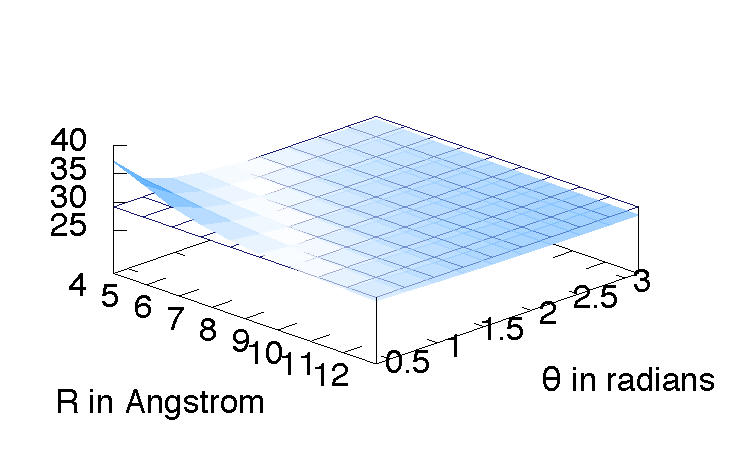
\includegraphics[scale=0.8]{pics/ArXeXe12_12_surf.pdf}
 \caption{Energy hyper surface of the doubly ionized
          ArXe5p$_{1/2}^{-1}$Xe5p$_{1/2}^{-1}$ (light blue) and the ionization
          potential of the Ar3s$^{-1}$ initial state with \unit[29.2]{eV}
          (dark blue). $Q$ is constant, whereas $R$ and the angle $\theta$
          (see figure \ref{}) are varied. This ETMD3 channel is open for
          structures where
          the final state energy is lower than the initial state energy.}
 \label{figure:ArXe2_geom_energy}
\end{figure}

At a hypothetical very small angle $\theta$ and $R\approx Q$, the channel closes.
In this example those geometries are mostly unrealistic, because the two xenon
atoms would be closer than in a neutral Xe dimer, but in other systems the
channel closing due to the geometry are to be expected.


\subsubsection{Geometry Dependence of the ETMD3 Decay Rates}
%\subsubsection{Distance Dependencies of ETMD Decay Rates}
The decay rate also crucially depends on the geometry of the triple.
From eq. (\ref{}) the $R$ dependency is easily interpreted of being
$\Gamma \propto R^{-6}$ corresponding to the energy transfer mainly being
caused by a dipole-dipole interaction. The dependency of $Q$ is implicitely
formulated in the transition dipole moments. These depend on the overlap
between the two atoms of the electron transfer, which decreases exponentially
with $Q$.



%\subsubsection{Angle Dependencies of ETMD Decay Rates}
The angular part of equation (\ref{}) can be reformulated using
the equivalence of transitions in $\tilde{x}$ and $\tilde{y}$ direction to
yield

\begin{equation}
  \Gamma_i \propto 2 \left( |<\tilde{D}_{z}>|^2 (1+\cos^2\alpha)
                           + |<\tilde{D}_x>|^2 (2+ \sin^2\alpha) \right)
\end{equation}

which are shown in figure \ref{figure:etmd_angle_dir}, supposing
$|<\tilde{D}_{z}>|^2 = |<\tilde{D}_x>|^2 = 1$.
Obviously the two different transition types add up to give the full
angular dependence of a given trimer. It has to be remembered, that
$|<\tilde{D}_{z}>|^2$ is about an order of magnitude larger than
$|<\tilde{D}_{x}>|^2$.

\begin{figure}[h]
 \centering
 \begin{tikzpicture}
    \begin{axis}[%scale=0.8,
                 domain=-0.5-pi:0.5+pi,
                 samples = 200,
                 xtick={-3.14159,-1.57089,...,3.14159},
                 xticklabels={$-\pi$,$-\frac \pi 2$,0,$\frac \pi 2$,$\pi$},
                 cycle list name = exotic,
                 legend style={anchor= north west}
                 ]
%    \foreach \q in {0.00,0.05,0.10,0.20,0.50}{
%      \addplot+[mark = none,
%               thick
%               ]
%               {4*\q + 2 + 2*cos(deg(x))^2 + 2*\q*sin(deg(x))^2}; 
%      \addlegendentryexpanded{$q=\q$}
%               }
      \addplot+[
                mark = none,
                thick
               ]
               {2*(1+cos(deg(x))^2)};
      \addlegendentry{$\tilde{z}$ direction};
      \addplot+[
                mark = none,
                thick
               ]
               {2*(2+sin(deg(x))^2)};
      \addlegendentry{$\tilde{x}$ direction};
      \draw[] (axis cs:\pgfkeysvalueof{/pgfplots/xmin},2) -- (axis cs:\pgfkeysvalueof{/pgfplots/xmax},2);
    \end{axis}
\end{tikzpicture}

 \caption{Angle dependence of the ETMD3 decay widths for electron transfers
          along the internuclear axis of subsystem $S_1$ $\tilde{z}$ and perpendicular
          to the internuclear axis $\tilde{x}$.}
 \label{figure:etmd_angle_dir}
\end{figure}

For a more realistic picture
consider the distances $R$ and $Q$ as definded in figure \ref{etmd_geom_pspic}
to be constant and the ratio between the transition dipole moments
in the $\tilde{z}$ and the $\tilde{x}$ direction
$q=\frac{|<\tilde{D}_x>|^2}{|<\tilde{D}_z>|^2}$ to be fixed to some number.
In this case the decay width for each $M_{AB}'$ has the angular dependence

\begin{align}
 \Gamma_i &\propto \left( 2q |<\tilde{D}_{z}>|^2 +
                  (4+2q)|<\tilde{D}_{z}>|^2 \cos^2\alpha +
                  (2+4q)|<\tilde{D}_{z}>|^2 \sin^2\alpha \right) \\
          &\propto 4q + 2 + 2 \cos^2\alpha + 2q \sin^2\alpha .
\end{align}

It is an oscillating function with maxima at even multiples of $\frac \pi 2$
and minima at uneven multiples at $\frac \pi 2$ as shown in figure
\ref{figure:etmd_angle}.

\begin{figure}[h]
 \centering
 \begin{tikzpicture}
    \begin{axis}[%scale=0.8,
                 domain=-0.5-pi:0.5+pi,
                 samples = 200,
                 xtick={-3.14159,-1.57089,...,3.14159},
                 xticklabels={$-\pi$,$-\frac \pi 2$,0,$\frac \pi 2$,$\pi$},
                 cycle list name = exotic,
                 legend style={anchor= north west}
                 ]
    \foreach \q in {0.00,0.05,0.10,0.20,0.50}{
      \addplot+[mark = none,
               thick
               ]
               {4*\q + 2 + 2*cos(deg(x))^2 + 2*\q*sin(deg(x))^2}; 
      \addlegendentryexpanded{$q=\q$}
               }
      \draw[] (axis cs:\pgfkeysvalueof{/pgfplots/xmin},2) -- (axis cs:\pgfkeysvalueof{/pgfplots/xmax},2);
    \end{axis}
\end{tikzpicture}

 \caption{Angular dependence of the \ac{ETMD}3 decay width for electrons trasnfers
          both along and perpendicular to the internuclear axis of subsystem $S_1$.
          Different values of $q=\frac{|<\tilde{D}_x>|^2}{|<\tilde{D}_z>|^2}$.}
 \label{figure:etmd_angle}
\end{figure}

In a real system, an energy transfer between
two dipoles is most efficient, if they are aligned in one direction.
Wihtin a dimer the most efficient electron transfer results in a
dipole aligned along the bonding axis and hence $q<1$. A typical
value of $q$ would be $\frac 1{10}$. In the 
case of $q$ approaching 0, the angular part of
the decay width
approaches a shifted $2\cos^2 \alpha$ with maxima at even multiples of $\frac \pi2$
and minima at uneven multiples of $\frac \pi2$ with values between
$4$ and $2$.
Therefore, for typical numbers of $q$ the energy transfer
to an atom on the same axis ($\alpha = 0,\pi$), corresponding
to a linear arrangement, is preferred.

The previous discussions are based on the decay of one specific atom
begin the electron donor and another atom being the electron emitter.
In reality both atoms can be donor als well as emitter while the energy
of the resulting final state stays the same. For both bond lengths to the
initially ionized atom being the same, both contribute the same decay rate
to the total decay rate. With one of the atoms ionized in the final state
being further apart, its probability in donating the vacancy filling electron
decreases exponentially and can hence be negliged.

\begin{figure}[h]
 \centering
 \begin{tikzpicture}
    \begin{axis}[scale = 0.8,
                 domain= 20:180,
                 y domain=4.0:15,
                 xtick={30,60,...,180},
                 cycle list name = exotic,
                 xlabel = {$\theta$},
                 ylabel = {$R$ [\AA]},
                 zlabel = {$\Gamma$ [eV]},
                 title = {ArXe5p$_{3/2}^{-1}$Xe5p$_{3/2}^{-1}$},
                 %view={0}{0}
                 view={230}{10}
                 ]
    \addplot3[surf,
             z buffer=sort
             ]
             table[
             x expr=\thisrowno{1},
             y expr=\thisrowno{0},
             z expr=\thisrowno{2}
             ]
             {data/ArXe2_etmd_surf.dat};
    \end{axis}
\end{tikzpicture}

 \begin{tikzpicture}
    \begin{axis}[scale = 0.8,
                 domain= 20:180,
                 y domain=4.0:15,
                 xtick={30,60,...,180},
                 cycle list name = exotic,
                 xlabel = {$\theta$ [$^{\circ}$]},
                 ylabel = {$R$ [\AA]},
                 zlabel = {$\Gamma$ [eV]},
                 title = {ArXe5p$_{3/2}^{-1}$Xe5p$_{1/2}^{-1}$},
                 %view={0}{0}
                 view={230}{10}
                 ]
    \addplot3[surf,
             z buffer=sort
             ]
             table[
             x expr=\thisrowno{1},
             y expr=\thisrowno{0},
             z expr=\thisrowno{3}
             ]
             {data/ArXe2_etmd_surf.dat};
    \end{axis}
\end{tikzpicture}
\\
 \begin{tikzpicture}
    \begin{axis}[scale = 0.8,
                 domain= 20:180,
                 y domain=4.0:15,
                 xtick={30,60,...,180},
                 cycle list name = exotic,
                 xlabel = {$\theta$},
                 ylabel = {$R$ [\AA]},
                 zlabel = {$\Gamma$ [eV]},
                 title = {ArXe5p$_{1/2}^{-1}$Xe5p$_{3/2}^{-1}$},
                 %view={0}{0}
                 view={230}{10}
                 ]
    \addplot3[surf,
             z buffer=sort
             ]
             table[
             x expr=\thisrowno{1},
             y expr=\thisrowno{0},
             z expr=\thisrowno{4}
             ]
             {data/ArXe2_etmd_surf.dat};
    \end{axis}
\end{tikzpicture}

 \begin{tikzpicture}
    \begin{axis}[scale = 0.8,
                 domain= 20:180,
                 y domain=4.0:15,
                 xtick={30,60,...,180},
                 cycle list name = exotic,
                 xlabel = {$\theta$},
                 ylabel = {$R$ [\AA]},
                 zlabel = {$\Gamma$ [eV]},
                 title = {ArXe5p$_{1/2}^{-1}$Xe5p$_{1/2}^{-1}$},
                 %view={0}{0}
                 view={230}{10}
                 ]
    \addplot3[surf,
             z buffer=sort
             ]
             table[
             x expr=\thisrowno{1},
             y expr=\thisrowno{0},
             z expr=\thisrowno{5}
             ]
             {data/ArXe2_etmd_surf.dat};
    \end{axis}
\end{tikzpicture}

 \caption{\ac{ETMD}3 decay widths $\Gamma$ hyper surfaces for an ArXe$_2$ trimer.
          The four electronic decay channels are shown separately.}
 \label{figure:ArXe2_etmd_geom_gamma}
\end{figure}

Combining both the view on the energetic accessibility of the decay
channels and the decay widths results in the pictures in
figure \ref{figure:ArXe2_etmd_geom_gamma}.
Here the geometry dependence of the decay width for the case of the four ArXe$_2$
channels is shown for all possible geometric combinations.
The numbers were obtained by \ac{HARDRoC} using the
asymptotic formula \ref{} with redefined $R$ and $\theta$. Here $Q$ is chosen constant
to the internuclear distance of the neutral ArXe dimer and $R$ and $\theta$
are varied. The plots exhibit the channel closing for very small Xe-Xe distances
and the $R^{-6}$ behaviour as well as the expected angle dependence explicitely
shown in figure \ref{figure:etmd_angle}. Implicitly the exponential decrease
of the decay width is shown by one of the two triple combinations in the trimer
showing a contribution only at small internuclear distances.

The decay widths of the four different decay channels shown in
figure \ref{figure:ArXe2_etmd_geom_gamma} can be summed up to yield
the total decay width of the ArXe$_2$ trimer as illustrated in figure
\ref{figure:ArXe2_etmd_geom_gamma_total}.

\begin{figure}[h]
 \centering
 \begin{tikzpicture}
    \begin{axis}[scale = 0.8,
                 domain= 20:180,
                 y domain=4.0:15,
                 xtick={30,60,...,180},
                 cycle list name = exotic,
                 xlabel = {$\theta$},
                 ylabel = {$R$ [\AA]},
                 zlabel = {$\Gamma$ [eV]},
                 title = {Total decay width of the ArXe5p$^{-1}$Xe5p$^{-1}$},
                 %view={0}{0}
                 view={230}{10}
                 ]
    \addplot3[surf,
             z buffer=sort
             ]
             table[
             x expr=\thisrowno{1},
             y expr=\thisrowno{0},
             z expr=\thisrowno{6}
             ]
             {data/ArXe2_etmd_surf.dat};
    \end{axis}
\end{tikzpicture}

 \caption{}
 \label{figure:ArXe2_etmd_geom_gamma_total}
\end{figure}

Also here the $R^{-6}$ dependence is observed but the dependency
of the angle $\theta$ looks spiky. These changes are due to the channel
closing. For a large angle $\theta$ all channels are open. Imagine a linear
trimer, which now starts bending. The closer
the two xenon atoms get, the more the two positive charges in the final
state repell each other. At one point the atoms are so close, that the
ArXe5p$_{1/2}^{-1}$Xe5p$_{1/2}^{-1}$ channel being highest in energy
is no longer energetically accessible. Bending further first the
ArXe5p$_{3/2}^{-1}$Xe5p$_{1/2}^{-1}$ and the
ArXe5p$_{1/2}^{-1}$Xe5p$_{1/2}^{-1}$ channels, being equal in energy,
close and finally also the ArXe5p$_{3/2}^{-1}$Xe5p$_{3/2}^{-1}$
channel.


\subsection{Influence of the Coordinate System Choice}
In section \ref{} a coordinate system was chosen to describe the
triatomic system. The distance $Q$ between the two atoms involved
in the energy transfer is reasonably defined. However, where the
center of the oscillating dipole moment of subsystem $S_1$ is, can
not unambigously be defined without further investigation. Most
probable it is somwhere between the atoms $A$ and $B$. Therefore
the center of mass was chosen to be the reference point for the
distance $R$ and associated with it the angle $\alpha$.
Another thinkable and for automatization of the calculation
convenient choice would be to anchorage $R$ and $\alpha$ at
atom $B$.
For the following discussion we will therefore refer to two sets
of coordinates of maximum deviation with origins residing in atoms
$A$ and $B$ with subscripts $A$ and $B$.

We assume that we have two constant distances $R_{A}$ and $R_B$
where either of these distances is larger than or equal to $Q$.
In this case the maximum and minimum of the ratio between the two
corresponding decay rates $\frac{\Gamma_{A}}{\Gamma_B}$ will occur
in the case of $\alpha = 0,\pi$ and $R_B = \frac 12 R_{A} = Q$
and $R_B = 2 R_{A} = 2Q$, respectively.

\begin{figure}[h]
 \centering
    \begin{tikzpicture}[scale=1.0,>=stealth]
%       \draw [help lines] (0,0) grid (10,7);
       
       \draw [very thick] (2,4) circle (0.3)
              node [name=A] {$A$};
       \draw [very thick] (2,2.5) circle (0.3)
              node [name=B] {$B$};
       \draw [very thick] (2,1) circle (0.3)
              node [name=C] {$C$};
       \draw [very thick] (A) -- (B);
       \draw [very thick] (B) -- (C);
       \path (A) edge [bend left] node [right] {$Q$} (B)
             (B) edge [bend left] node [right] {$R_B$} (C)	
             (A) edge [bend right] node [left] {$R_A$} (C);

    \begin{scope}[xshift=5cm]
       \draw [very thick] (2,4) circle (0.3)
              node [name=A] {$A$};
       \draw [very thick] (2,2.5) circle (0.3)
              node [name=B] {$B$};
       \draw [very thick] (2,5.5) circle (0.3)
              node [name=C] {$C$};
       \draw [very thick] (A) -- (B);
       \draw [very thick] (A) -- (C);
       \path (A) edge [bend right] node [left] {$Q$} (B)
             (B) edge [bend right] node [right] {$R_B$} (C)	
             (A) edge [bend left] node [left] {$R_A$} (C);
    \end{scope}

   \end{tikzpicture}

 \caption{}
 \label{}
\end{figure}

\begin{equation}
\text{minimum: } \frac{\Gamma_{A}}{\Gamma_B}= \frac{1}{64} \quad\quad
\text{maximum: } \frac{\Gamma_{A}}{\Gamma_B}= \frac{64}{1}
\end{equation}

From this we conclude, that the absolute numbers of calculated ETMD
decay widths are obviously error-prone. In the worst case the uncertainty
is given by factors $\frac{1}{64}$ or $\frac{64}{1}$.
In reality these worst cases will rarely be observed, since it on
the one hand is very unlikely to find two atoms at exactly the same place
and on the other hand ETMD preferably occurs at interfaces, which leads
to preferred angles higher than 0 and below $\pi$.
Additionally the larger the difference between $Q$ and $R$ become, the
smaller this effect is going to be.


\subsection{Relative Decay Rates Depending on the Symmetry of the Final States}

\chapter[Heteroatomic Noble Gas Clusters]{Competing Processes in Heteroatomic Noble Gas Clusters}
\label{chapter_clusters}

The modelling of secondary electron spectra stemming from \ac{ICD}
and \ac{ETMD}3 processes are carried out using the programme
HARDRoC \cite{HARDRoC}, which is based on the model of pairs and
triples explained in chapter \ref{chapter:geom} and is applied
to a given cluster structure. The obtained
decay widths are proportional to the probability of the underlying decay.
The experimental spectra are obtained from a multitude of distinct measurements.
Hence, for a reasonable large number of measurements, a distribution with the
same statistical behaviour as for the decay width calculation in the
model of pairs and triples is achieved. Therefore, the experimental spectra
can be directly compared with the theoretically obtained spectra.

For the actual calculation the energies of the secondary electrons are obtained
from equation \ref{equation:E_sec}. The single ionization energies
can be obtained in two different ways. They can be
approximated by the atomic ionization energies in Table
\ref{table:noble_atom_properties} corrected by energetic shifts
given in Table \ref{table:cluster_shifts} in order to take
the effect of the cluster environment into account. 
Alternatively, they can be taken from the single ionization spectrum
measured at the same time and the same conditions as the electron-electron
coincidence experiment. The latter is to be preferred, since the energy shifts
of Table \ref{table:cluster_shifts} are obtained from homonuclear clusters and
hence only give a first approximation to the real energetic shift in
heteronuclear cluster. Since both the \ac{ICD} and even more clearly the
\ac{ETMD}3 occur at the interfaces, it is crucial for a good modelling to
describe the ionization energies of these atoms as accurate as possible.

The decay widths $\Gamma$ can either be obtained from the asymptotic expressions
in equations (\ref{reltheolifetime_exp}) and (\ref{reltheolifetimeetmd_exp})
using the atomic properties given in Table \ref{table:noble_atom_properties}
or from a fit to decay widths obtained from FanoADC-Stieltjes calculations.

In the following sections two different heteronuclear clusters are investigated
illustrating different effects on the secondary electron spectra.
In the case of ArXe clusters I will focus on the effects of spin-orbit coupling
on the secondary electron spectra. Furthermore, I will investigate the influence
of the cluster size and number of argon shells around the xenon core and
the influence of the basic structure of the cluster and show the
difference of the spectra
obtained from clusters having an icosahedral
and \ac{fcc} structure.
In the case of NeAr clusters I will focus on the bidirectional dependence of
the ICD spectra of the competing NeNe-ICD and NeAr-ICD processes and
different arrangements of neon atoms around the argon core.

\newpage

\begin{figure}
 \centering
 \input{pics/exp_309ico_arxe}
 \caption{}
 \label{exp_309ico_arxe}
\end{figure}



\begin{figure}
 \centering
 \input{pics/exp_923ico_arxe}
 \input{pics/exp_923fcc_arxe}
 \caption{}
 \label{exp_923ico_arxe}
\end{figure}

%\begin{figure}
% \centering
% \input{pics/exp_923fcc_arxe}
% \caption{}
% \label{exp_923fcc_arxe}
%\end{figure}

\newpage
\section{Structure Determination of NeAr Clusters}

In general, the structure determination of heteronuclear noble gas
clusters is an unsolved problem. However, the maximization of the cohesive
energy suggests a core of argon atoms surrounded by neon atoms.
Electron-electron coincidence experiments proved their existence by the
presence ICD electron from NeAr-ICD processes \cite{Lundwall07}.

The clusters consist of neon and argon atoms. Since an inner-valence vacancy in
the Ne2s can decay both via NeNe-ICD and NeAr-ICD, both competing processes
are expected to be observed in an experiment. In the literature most
investigations focussed on the NeAr-ICD, because it, until recently, was not
possible to measure the NeNe-ICD as well \cite{Fasshauer14_1}.
From these studies, large NeAr clusters established by coexpansion and
consisting of an argon core with
approximately 1000 atoms were determined to have a core-shell structure
\cite{Lundwall07,Barth_diss}
and to have a temperature of \unit[40 -- 50]{K} \cite{Barth_diss}.
In his PhD thesis, Barth suggested the possibility to gain information about
the cluster structure from the efficiency of the NeAr-ICD compared to the
total decay of the Ne2s ionization. This was proposed to be possible, since
the sum over the NeNe-ICD and NeAr-ICD previously had been shown to
cause almost the total decay of the Ne2s vacancy \cite{Marburger_diss}.
The results indicated an increasing NeAr-ICD efficiency with increasing
cluster size and hence a smaller surface-to-bulk ratio.

This structure determination, as is going to be shown, is indeed possible
because the decay widths of the competing NeNe-ICD and NeAr-ICD processes
are of the same order
of magnitude and therefore both signals are observable. Additionally, as shown
in the preceeding section about ArXe clusters, the secondary electron spectrum
crucially depends on the underlying structure.

Recently, the NeNe-ICD in NeAr clusters could be measured. Therefore, I will
present the structure determination of NeAr clusters from ICD electron
spectra by comparison of experimental spectra with theoretical calculations.

The chapter is structured as follows: First, the experimental results are
presented and the computational details for the simulation of the ICD
electron spectra are demonstrated. Afterwards, the manifold of different 
hypothetical cluster structures are introduced. Finally, the comparison
between the experimental findings and theoretical predictions will be used
for the determination of mean cluster structures.


\subsection{Experimental Results}
Recently, it was possible to measure the full secondary electron spectrum
of NeAr clusters under different experimental conditions as shown in Figure
\ref{figure:NeAr_exp_spectrum} and Table \ref{table:expansion_conditions}.

\begin{figure}[h]
  \centering
  \includegraphics[scale=1.7]{pics/exp_near_coinc_sets.eps}
  \caption{Electron-electron coincidence spectra for NeAr clusters
           showing both NeNe-ICD and NeAr-ICD signals \cite{Fasshauer14_1}.}
  \label{figure:NeAr_exp_spectrum}
\end{figure}

\begin{table}[!h]
 \centering
 \caption{Assignment and expansion parameters of the five different
          cluster ensembles. Included are also the resulting mean
          cluster sizes calculated for the homogeneous species according
          to the formalism intruduced by Hagena \it{et al.}
          \cite{Hagena72}}
  \begin{tabular}{c c c c c c}
          \toprule
           designation    &       Ar content in   & expansion & nozzle & $\langle N\rangle _{Ne}$ & $\langle N\rangle _{Ar}$ \\
                                          &       initial mixture &  pressure & temperature & &  \\
          \midrule
          Set 1   &       \unit[1.7]{\%}  &       \unit[0.26]{bar}        &       \unit[63]{K}    &       \unit[5]        &       \unit[520]      \\
          Set 2   &       \unit[7.4]{\%}  &       \unit[0.40]{bar}        &       \unit[60]{K}    &       \unit[17]       &       \unit[1850] \\
          Set 3   &       \unit[1.7]{\%}  &       \unit[0.25]{bar}        &       \unit[57]{K}    &       \unit[7]        &       \unit[810]  \\
          Set 4   &       \unit[7.4]{\%}  &       \unit[0.24]{bar}        &       \unit[58]{K}    &       \unit[6]        &       \unit[670]  \\
          Set 5   &       \unit[1.0]{\%}  &       \unit[0.16]{bar}        &       \unit[54]{K}    &       \unit[3]        &       \unit[380]  \\
          \bottomrule
  \end{tabular}
\label{table:expansion_conditions}
\end{table}

The spectra have been normalized to the peak height of the NeAr-ICD signal.
It can clearly be seen that for different experimental conditions the
size of the NeNe-ICD peak varies compared to the NeAr-ICD peak as explicitely
listed in Table \ref{table:clustervalues}. This can be
explained both by different cluster sizes and by different cluster structures
as I am going to show in this thesis. Both the main NeNe-ICD and the NeAr-ICD peak
have a shoulder at higher energies. For NeAr dimers such a structure has
been proposed to potentially stem from vibrations. However, such bound vibrational
states above the ground state do not exist in neon dimers. I am going to show
that this peak structure can be related to \ac{ICD} processes with next nearest
neighbours. Still, excitations to higher vibrational states might contribute
to the peak structure as well.

\begin{table}[!h]                                                                                                                                       
 \centering                                                                                                                                      
 \caption{Experimental results. Percentaged values are contributions to the
          respective total values. The cluster band onsets are given
          at half the peak height of the respective feature.}
   \begin{tabular}{c c c c c}                                                                                                              
           \toprule
            designation    &       Ar content in   & onset Ar3p                    & onset Ne2p            & Ne-Ar ICD     \\
                                           &       final cluster   &   cluster band                & cluster band          & contribution  \\
           \midrule
           Set 1   &       \unit[47 $\pm$ 10]{\%}  &       \unit[14.7$\pm$ 0.1]{eV}        &       \unit[20.93$\pm$ 0.08]{eV}      &       \unit[63 $\pm$ 7]{\%}   \\
           Set 2   &       \unit[35 $\pm$ 5]{\%}   &       \unit[14.6$\pm$ 0.1]{eV}        &       \unit[20.86$\pm$ 0.08]{eV}      &       \unit[61 $\pm$ 10]{\%}  \\
           Set 3   &       \unit[21 $\pm$ 4]{\%}   &       \unit[14.8$\pm$ 0.1]{eV}        &       \unit[20.86$\pm$ 0.08]{eV}      &       \unit[38 $\pm$ 5]{\%}    \\
           Set 4   &       \unit[20 $\pm$ 4]{\%}   &       \unit[14.8$\pm$ 0.1]{eV}        &       \unit[20.86$\pm$ 0.08]{eV}      &       \unit[53 $\pm$ 6]{\%}    \\
           Set 5   &       \unit[8 $\pm$ 2]{\%}    &       \unit[15.0$\pm$ 0.1]{eV}        &       \unit[20.89$\pm$ 0.08]{eV}      &       \unit[28 $\pm$ 3]{\%}    \\
           \bottomrule
   \end{tabular}
\label{table:clustervalues}                                    
\end{table}




\subsection{Computational Details}
The energies of the secondary electron were calculated using the
experimentally obtained ionization energies given in Table \ref{exp_input}.

\begin{table}[h]
 \caption{Experimental values used for the estimation of the decay widths
          \cite{Fasshauer14_1}.}
 \label{exp_input}
 \centering
 \begin{tabular}{lc}
  \toprule
  indicator            &  value \\
  \midrule
  SIP(Ne2s)            &  \unit[47.75]{eV} \\
  SIP(Ne2p)            &  \unit[21.10]{eV} \\
  SIP(Ar3p)$_{c<3}$    &  \unit[15.40]{eV} \\
  SIP(Ar3p)$_{c\ge 3}$ &  \unit[15.20]{eV} \\
  \bottomrule
 \end{tabular}
\end{table}

The distance dependence of the NeAr dimer was non-relativistically calculated with
the Fano-Stieltjes procedure implemented in Dirac \cite{DIRAC13,Fasshauer14_2}
with an aug-cc-pV6Z basis set on both atoms. 
Additional basis functions of five $s$, $p$ and $d$ functions each of the
KBJ type \cite{Kaufmann89} were introduced on a ghost atom in the
geometric center of the dimer.

Since inversion symmetry is until now not treated correctly,
for the neon dimer decay width data from the literature is used, which was
obtained with the same method and a comparable basis set \cite{Averbukh06_1}.
The resulting decay widths are shown in Figure \ref{figure:fitted_NeAr_widths}
and the corresponding lifetimes are in Table \ref{table:NeAr_gammas} compared
to other values from the literature.

\begin{table}[htb]
 \centering
 \caption{Decay widths of the NeNe-ICD and NeAr-ICD obtained
          using different theoretical
          methods and from experiment.}
 \begin{tabular}{lcrcrcr}
  \toprule
        & \multicolumn{2}{c}{Theory used} & \multicolumn{2}{c}{Theory Comp.} & \multicolumn{2}{c}{Experiment} \\
  \midrule
   NeNe & \unit[60.4]{fs} & \cite{Averbukh06_1} & \unit[92]{fs} & \cite{Vaval07} & \unit[$150\pm 50$]{fs} & \cite{Schnorr13}\\
   NeAr & \unit[44.2]{fs} & This work & \unit[36]{fs} & \cite{Scheit06} &  --  &\\
  \bottomrule
 \end{tabular}
 \label{table:NeAr_gammas}
\end{table}

The NeAr-ICD has a higher decay width than the NeNe-ICD, but since the
actual value of the decay width strongly depends on the method and basis set
used for its description, larger discrepancies are normal. For the decay
width estimation of the NeAr clusters the values of the first column were
chosen, because they were both calculated using the FanoADC-Stieltjes approach
with comparable basis set size.

\begin{figure}[h]
 \centering
 \input{pics/NeArfit_pgf}
 \caption{Decay widths of the NeNe-ICD and NeAr-ICD processes fitted to
          curves for the decay width estimation of the NeAr clusters.}
 \label{figure:fitted_NeAr_widths}
\end{figure}

For each structure defined in the following section the NeNe-ICD and NeAr-ICD
spectra were calculated using the programme HARDRoC \cite{HARDRoC}.




\subsection{Hypothetical, idealized structures of the NeAr clusters}

It is known that small noble gas clusters preferably form icosahedral structures,
while with increasing cluster size a fcc structure becomes more favorable. This transition
occurs at cluster sizes in the range from 750 to 3500 atoms \cite{Martin96,Doye97,Hartke02}.
For the simulations it is assumed that the clusters of all
five experimental cluster sets have 
icosahedral structure. For all sets but set 2 the expansion conditions should result in clusters 
with mean sizes below 750 (see Table \ref{table:expansion_conditions}). Still,
the mean size of the clusters of set 2 is well below 3500.

\begin{figure}[!ht]
 \centering
 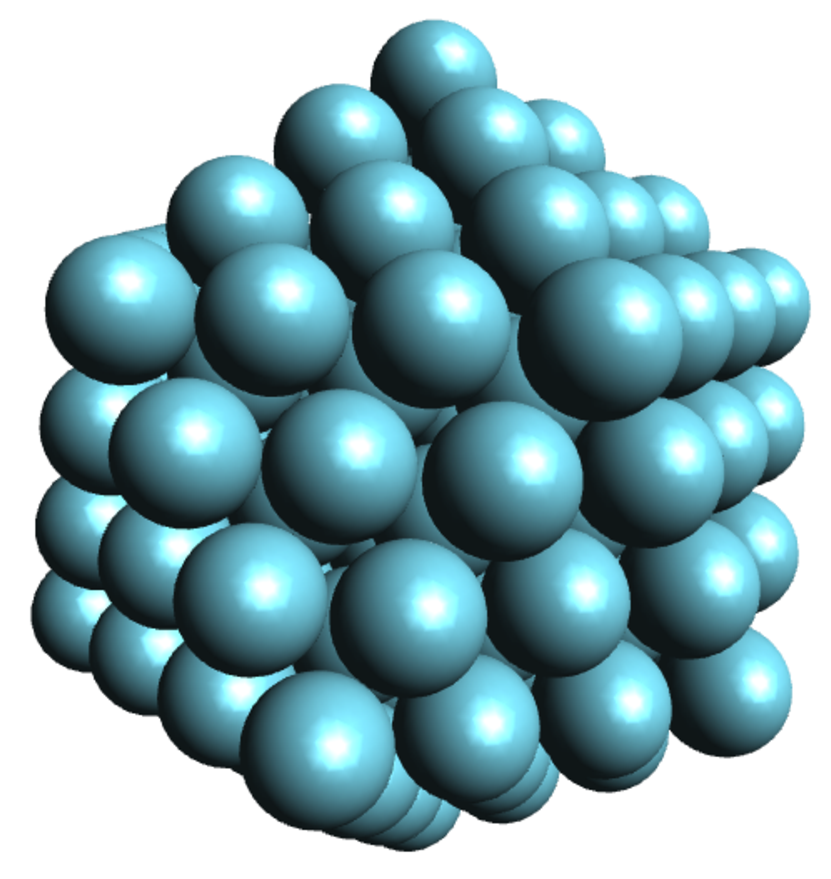
\includegraphics[scale=0.5]{pics/Ar_pure.eps}                        
 \caption{An icosahedral argon cluster with an edge consisting of 
          $c=\unit[4]{atoms}$, containing \unit[147]{atoms},
          distributed over four shells. \unit[55]{atoms} belong
          to the core, 12 are at the vertices, 60 in the edges and 20 inside the
          surfaces.}
 \label{figure:Ar_pure}
\end{figure}    

The actual cluster formation process is understood as follows. First, a three particle
collision has to take place to form argon dimers. Subsequently, single atoms are added to the dimer 
due to collisions. At a later stage these clusters can also collide to form larger clusters. This process,
called coagulation, becomes the dominant process for the formation of very large clusters. 
The experiment of Lundwall et al. \cite{Lundwall07} was interpreted to
show clusters consisting of an argon core with distinct, complete neon
shells around it, which is plausible, since according to the sum of van der Waals
energies, this should be the most stable kind of clusters.
Therefore this structure is chosen as a starting point for the considerations
about the average structure of the clusters.

In all structures considered throughout this thesis the core is build as
 an icosahedral
structure of argon atoms as shown in Figure \ref{figure:Ar_pure}.
In this example, it has an edge length
of $c=\unit[4]{atoms}$ and consists of $n_{Ar}=\unit[147]{atoms}$, which can be
calculated as \cite{Martin96}

\begin{equation}
  n_{atoms} = \frac{10}{3} c^3 - 5 c^2 + \frac{11}{3} c -1 .
\end{equation}

For the construction of the structure the minimum
distance between two argon
atoms is assumed to be twice the van der Waals
radius of argon $r_{Ar}=$ \unit[1.88]{\AA} \cite{Bondi64}. In order to abide by this
minimum distance in the case of two atoms in a surface position in different
shells, the distance of two atoms in the edges is slightly increased.

As is going to be seen in the discussion, the outcome of the experiment
cannot completely be explained by an argon core surrounded by complete neon shells.
This leads to considerations of other structures with an argon core somehow surrounded
by neon atoms. These are divided into three types, so that, in total, four
different classes of cluster structures are studied as
shown in Figure \ref{figure:structures}:

\begin{enumerate}
 \item complete shells
 \item incomplete shells around complete shells
 \item caps
 \item randomly arranged neon atoms around complete shells
\end{enumerate}

\begin{figure}[h!]
 \centering
 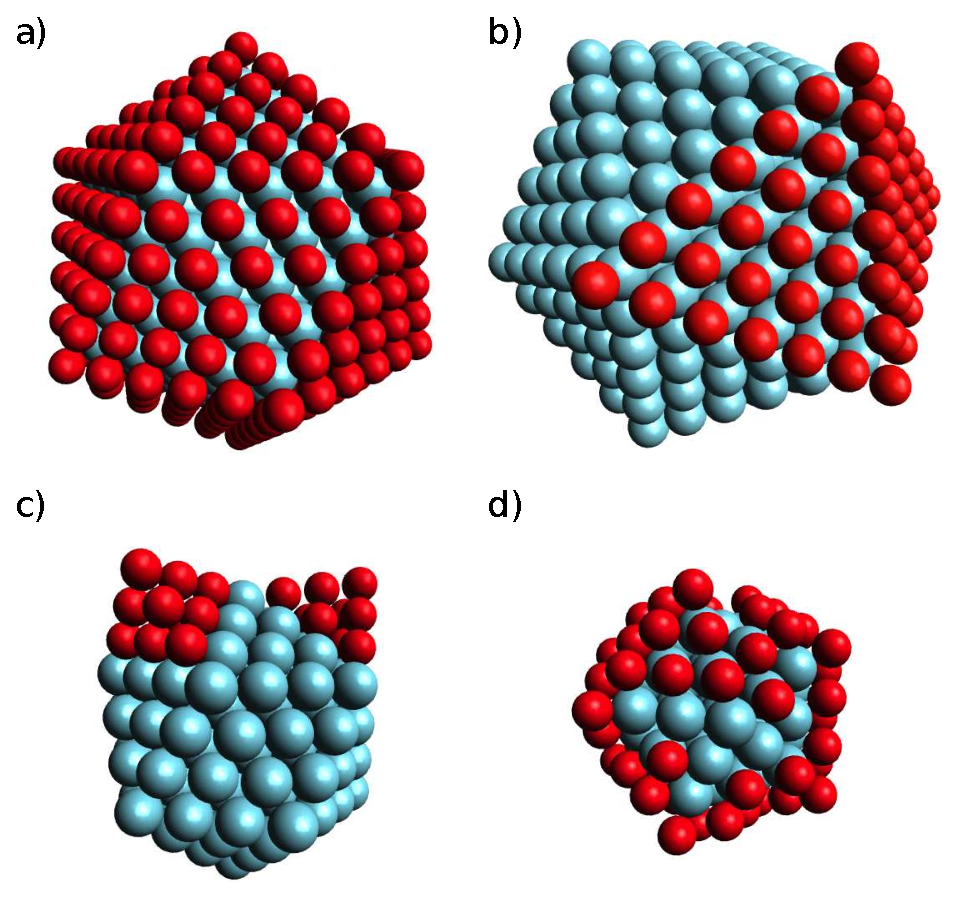
\includegraphics[scale=0.9]{pics/NeAr_structures1.eps}
 \caption{Structure classes considered in our calculations.\\
          a) complete shells, in this example $c=\unit[5]{atoms}$ with one layer
          neon atoms,\\
          b) incomplete shells, in this example
          $c=\unit[6]{atoms}$ with two covered trinangular surfaces
          of neon,\\
          c) caps, in this example $c=\unit[4]{atoms}$ with two caps,\\
          d) randomly arranged neon atoms around a full shell cluster,
          here $c=\unit[3]{atoms}$ directly covered by neon atoms
          with an argon content of \unit[47]{\%}.}
 \label{figure:structures}
\end{figure}

In the case of an argon cluster with one or more complete shells of neon
atoms around it, first the core structure is created and afterwards the
outer shells are constructed around it, such that the minimum distance between a
neon atom in the surface and an argon atom in the shell beneath is the sum
over the van der Waals radii, where $r_{Ne}=$\unit[1.54]{\AA} \cite{Bondi64}
(see Figure \ref{figure:structures} panel a).

Not all experimentally determined argon contents in the mixed clusters
fit to complete neon shells. Maintaining the idea of shells,
the possibility of incomplete shells is considered.
The cluster structures are created analogously to the
complete shells except that not all triangular surfaces areas of the argon core
are covered by neon atoms (for an example see Figure \ref{figure:structures}
panel b).

Another possibility is caps covering surface areas as shown
in Figure \ref{figure:structures} panel c. These structural elements
do not lead to minimum energies for clusters, but they might explain a
large number of neon-neon interactions compared to the number of
neon-argon interactions in the experiments.
The neon-neon distances within the caps are
calculated in the same
manner as described before for the (in-)complete shells.
A whole manifold of different positionings of several caps are in principle
possible, but calculations showed, that these different
placements of caps did not change the ratios of NeAr- to NeNe-ICD for a
constant number of caps. Since these structures cannot be distinguished
by ICD spectra, the
discussion is limited to structures containing different numbers of caps.

One could also think about neon atoms randomly arranged around a homonuclear
or heteronuclear cluster with complete shells and randomly attached neon
atoms around it as shown in Figure \ref{figure:structures} panel d.
It is constructed as a cluster with complete shells and afterwards adding
neon atoms in random positions of the next layer until the requested
$n_{Ar}/n_{Ne}$ ratio is reached.

All these structures are idealized and highly symmetric, which reduces
the computational cost. They were constructed using the set of \verb|icoclus|
scripts written for this purpose and explained in the
appendix \ref{section:icoclus}.
Vibrations inside the clusters will change the interatomic
distances and hence both the kinetic energies of the ICD electrons as well as
the decay widths. As has been shown for NeAr \cite{Scheit06}, the ICD processes
are faster than dynamical rearrangements, caused by Coulombic attraction
after the initiating ionization, or vibrations. In case of the neon dimer, the
ICD lifetime is of comparable size to the rearrangement time and hence
influences the ICD electron spectra \cite{Scheit03}. However, in clusters, the
initially ionized atom interacts with more than one other atom, which leads
to more neighbours it can undergo ICD with. Hence, the decay width increases
to first approximation linearly with the number of nearest neighbours.
At the same time, the larger number of neighbours stabilizes the position
of the initially ionized atom in space compared to the dimer.
Therefore, it is assumed that the structures given above are good
approximations to the decaying clusters.




\subsection{Interpretation of the graphs}

In order to have comparable numbers, for the theoretical estimations and
experimental results the entities chosen for the characterization of each
cluster structure and measurement are
the argon content in the cluster and the amount of
NeAr-ICD compared to the total ICD
$\frac{\Gamma_{NeAr}}{\Gamma_{NeAr}+\Gamma_{NeNe}}$.
Throughout the thesis, the same 
colour coding as for the experimental spectra
shown in Figure \ref{figure:NeAr_exp_spectrum} is used,
for which the numbers are listed in Table \ref{table:clustervalues}.
The results are going to be plotted as in Figure \ref{figure:incompl01_02_explain}.
As an example, the results for clusters of the class of an
incompletely filled neon shell
around an argon core with a an edge size of $c=2$
surrounded by one complete shell of neon atoms are shown.
Here, the ratio of NeAr-ICD to total ICD is plotted against the argon content
of the cluster. The results of the five different experimental conditions and their
errors are shown by the coloured areas, where the colour corresponds to the
set with the same colour as in Figure \ref{figure:NeAr_exp_spectrum}.
Additionally plotted are the theoretical results for the different structures
parted into first the classes of the structures and secondly by the size of the argon core.
The higher the argon content is, the less of the 20 surfaces of the underlying
complete shell is covered by either layer(s) or caps. The easiest way to interpret
the graphs is to start from a complete shell and then covering one surface. This
corresponds to the rightmost theoretical value within a group. Each step further
to the left refers then to one more covered layer with either caps or layers.\\

\begin{figure}[!h]
  \centering
  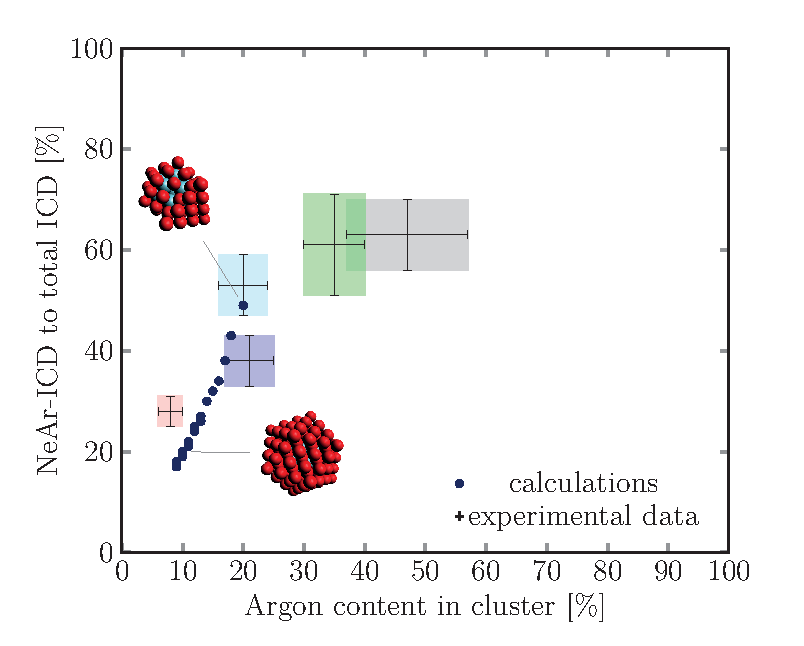
\includegraphics[scale=0.75]{pics/incompl01_02_mit_inlays.eps}
  \caption{NeAr-ICD to total ICD ratio plotted against the argon content
           in the cluster for both experimental results for all five sets of
           conditions as well as theoretical calculations for cluster structures
           with an incomplete outermost shell surrounding an argon core of
           $c=2$ and one additional complete neon shell. For illustrative purposes,
           pictures of two structures are included at their respective
           theoretical values.}
  \label{figure:incompl01_02_explain}
\end{figure}

By looking for agreements of theoretical and experimental values
possible structures are deduced.
The agreements between experimental and theoretical results are evaluated
using the graphical distance from the experimental results
\begin{equation}
  d = \sqrt{\Delta_{Ar}^2 + \Delta_{\Gamma}^2}    ,
\end{equation}
where $\Delta_{Ar}$ and $\Delta_{\Gamma}$ denote the deviation of the argon content
and the ratio of NeAr-ICD decay width and the total decay width, respectively.
Only such structures are considered, where the argon content of the model
structure lies within the error range of the experimental findings.


\subsection{Assignment of the different measurements to cluster structures}
For the assignments the following criteria are used:

\begin{itemize}
 \item onsets of single ionization potentials for the determination
       of the size of the argon core
 \item positions of NeAr-ICD peak
 \item relative expected mean cluster sizes
       (see Table \ref{table:expansion_conditions})
 \item agreement of predicted and measured ICD (see Table \ref{table:assignments})
\end{itemize}

From the onsets of the single ionization potentials and the position of the
NeAr-ICD peak at a lower energy it is deduced that the mean argon core of set 5
is the smallest of all measured ensembles. Since the nearest neighbours have
the largest influence of such a shift these clusters can be interpreted to have
an edge length of either $c=1$ or $c=2$.\\
Since the estimations of mean cluster sizes based on Hagena refer to expansions
of only one atom type, only the results with the same argon content should
be compared. From this the core of set 2 can be expected to be bigger than the core
of set 4 and the core of set 3 can be expected to be slightly larger
than the core of set 1.
These estimations do not have to resemble the final conclusions, since the
approach is only valid for homogeneous clusters, but can give hints
in the following procedure. The assignment due to geometrical distance
of the predicted results from the experimental counterparts is to be found in
Table \ref{table:assignments}. There, the best results for all sets are shown
in the following way: $c$ depicts the number of atoms in the longest edge
of the argon core, which is then covered by a number of additional complete
neon shells with additional covered triangular surfaces or randomly arranged atoms
and $d$ denotes the geometrical distance.

\begin{table}[!h]
  \caption{The smallest geometric distances for each set of clusters
           and the corresponding cluster structures.
           Note that for set 4 only the random arrangement is listed,
           for which the argon content exactly equals the experimental one.}
  \centering
  \begin{tabular}{lccccc}
    \toprule
     Set  & $c$ & complete Ne shells & covered surfaces & random & $d$\\
    \midrule
      1   & 4   &          1         &        1         &   -    & 2.000\\
      1   & 5   &          1         &        2         &   -    & 4.472\\
      1   & 2   &          0         &        5         &   -    & 4.472\\
    \midrule
      2   & 3   &          1         &        -         &   x    & 1.000\\
      2   & 3   &          1         &        1         &   -    & 3.162\\
      2   & 2   &          0         &        8         &   -    & 4.123\\
    \midrule
      3   & 2   &          1         &        3         &   -    & 4.000\\
      3   & 3   &          1         &        7         &   -    & 4.123\\
      3   & 3   &          1         &        8         &   -    & 4.472\\
    \midrule
      4   & 2   &          1         &        -         &   x    & 2.000\\
      4   & 2   &          1         &        1         &   -    & 4.000\\
    \midrule
      5   & 2   &          1         &       13         &   -    & 8.246\\
      5   & 2   &          1         &       14         &   -    & 9.220\\
      5   & 2   &          1         &       15         &   -    & 9.220\\
    \bottomrule
  \end{tabular}
  \label{table:assignments}
\end{table}

The structure assignment is going to be discussed in descending order
of the set number, which more or less corresponds to a discussion with
increasing size of the clusters.\\
The assignment is started with set 5 (red). As already mentioned,
these clusters can be expected
to be small and, additionally, the smallest ones measured. These expectations are
in agreement with the results of Figure \ref{figure:incompl01_02_explain}
(also to be found in the
appendix in Figure \ref{incompl01-core02}), where the red square
can be matched with a cluster to an argon core with $c=2$, one complete
shell of neon atoms 
and one almost complete
shell with 13 -- 20 out of 20 surfaces covered by neon atoms. None of the
theoretical estimates coincide with the experimental findings. This might be
explained by even smaller clusters not showing an icosahedral argon core, but
a coagulation of 2--11 atoms plus some neon atoms.

Set 4 (turquoise) shows a very good agreement for a structure with $c=2$ with one
complete shell of neon atoms and some additional atoms (see Figures
\ref{random-core02} and \ref{incompl01-core02} or in the example above).
Whether these atoms are
randomly arranged around the complete shells or are to be found together cannot
finally be decided. From the geometric distance, the random arrangement should
be preferred.

The results of set 3 (blue) shows a good agreement with structures
of $c=2$ or $c=3$ surrounded by one complete shell of neon atoms and additional
neon atoms covering 3 or 7 -- 8 triangular surfaces, respectively 
as shown in Figures \ref{incompl01-core02} and \ref{incompl01-core03}. 

With the two latter assignments it is possible to distinguish
the structures of two cluster manifolds with the same argon content by utilizing the
ICD spectra.

Set 2 (green) can be assigned to core sizes of $c=2-3$ plus further neon atoms
(see Figures \ref{incompl00-core02} and \ref{incompl01-core03}).
In the case of $c=3$, one additional complete shell of neon atoms fits
best to the experimental results, but as for set 4 the arrangement as such for
some few additional atoms can either be random or coagulated.
In case of $c=2$ the best fit holds for no additional complete shell of
neon atoms but with 8 triangular surfaces covered, the shell is almost halfway filled.
Further structures with larger core sizes as $c=4$
are also quite probable. Considering, that 
both from Hagena's approach and the single ionization potential
onsets of the Ar3p band, set 2 is supposed to have the largest mean structure
core, the latter structures might be closer to reality than the ones of the small clusters
with $c=2,3$.

Due to the large error bars, set 1 (black) can be assigned to a whole manifold
of different structures with $c = 2 - 6$ within the error bars
either with caps or, more probably,
with about one complete shell of neon atoms, plus maybe additional covered surfaces
or randomly surrounded by neon atoms. Since caps should be energetically less
favourable than the other structures, I will suspend those structures
and concentrate
on the rest.
From Hagena's approach I concluded that the core of the clusters of set 1
should be slightly
smaller or of comparable size as the clusters from set 3. Therefore I assume
the average cluster structure to consist of an argon core of $c=2-4$ shells
with one complete neon shell and possibly one further incomplete shell, of
which I cannot give more detailed information.

One might have to consider completely different structures not investigated in this
thesis. Formed, mixed clusters might collide and coagulate, yielding
structures impossible to be estimated by a core-shell structure of the kinds
presented in this work. 

From the best agreement of the calculated NeAr-ICD to total ICD ratios listed in Table
\ref{table:assignments}, the corresponding estimated spectra are folded
with gaussians with a width of \unit[250]{meV}
and are plotted in Figure
\ref{figure:theo_specs}.
From these spectra and the underlying calculations
I conclude, that the shoulders of both the NeNe-ICD and the NeAr-ICD peak
at \unit[2.5--4]{eV} and \unit[8--10]{eV}
correspond to next-nearest neighbours inside the clusters, while the differences
in the main peak stem from almost equal interatomic distances but different positions
in the cluster such as corner, edge or surface.\\
The main peaks of the NeNe-ICD correspond well with the experimental observations
of Figure \ref{figure:NeAr_exp_spectrum}.\\
The onset of the NeAr-ICD peak depends on the shielding of the argon atom
and hence the cluster size. For set 5 the assignment seems to be correct, while
for set 4, the experiment shows a higher energy of the ICD electron. 
This deviation implies that either the core of the mean cluster structure
is larger than evaluated from the theoretical calculations or that
the choice of $c=3$ as the minimum core size for the for the lower ionization
potential of the Ar3p was wrong.
The truth, however, is not a spontaneous jump from one shell to the other, but rather a decrease
with more and more atoms. If one is interested in clusters of $c\le2$ only, one
should take care of a more detailed description of the different ionization
potentials for different cluster sites.

\begin{figure}[!ht]
  \centering
  \input{pics/near_clusters/spec-250meV}
  \caption{Calculated ICD electron spectra for those structures given in Table
           \ref{table:assignments} with the best agreement to the experimental
           argon content and NeAr-ICD to total ICD ratio. The intensities are given
           in arbitrary units and are normalized to the peak height of the NeAr-ICD
           peak and the spectra are folded by Gaussians with widths of \unit[250]{meV}.
           The theoretically calculated specrta nicely match the experimental ones in Figure
           \ref{figure:NeAr_exp_spectrum}.
           Both, the NeNe-ICD peak at low energies and the NeAr-ICD peak
           at higher kinetic energies, show a peak structure which can be related
           to different distances of the atoms involved in the process within the
           clusters. For more details, see the text.}
  \label{figure:theo_specs}
\end{figure}

\subsection{Conclusions}
I have developed a method for the analysis of a mean cluster
structure of noble gases utilizing the relative ICD decay widths
of two competitive decay processes. This I have exploited onto
five different cluster ensembles. I am able to explain the
spectra by different underlying mean structures. From the results I conclude, that
clusters formed in a supersonic beam most likely can be described
by a core-shell structure with additional layers. In some limited cases,
when only few additional neon atoms around complete shells are needed
to fulfill the argon content, the random arrangement seems to be possible.\\
%It is to be investigated, whether this method opens a possible structure
%analysis for distiguishing an underlying icosahedral structure from a
%crystal like fcc one.




\chapter{Summary and Outlook}

In this thesis, the importance of relativstic effects on autoionization
processes, especially \ac{ICD}-like
processes, and cluster environments have been discussed.
For this purpose, asymptotic expressions for the relativistic decay width of the ICD
and both, relativistic and non-relativstic asymptotic expressions for the ETMD3
have been derived. Additionally, the non-relativistically known
FanoADC-Stieltjes approach
using a partitioning of the Hamiltonian by 2h configurations has been implemented
in the relativistic programme package \verb|DIRAC| \cite{DIRAC13},
which allows for the
description of decay width including relativistic effects.
In order to model the experimental secondary electron spectra of noble gas
clusters, the model of pairs and triples was introduced and automatized in the
programme \verb|HARDRoC| \cite{HARDRoC}. It enables the estimation of
decay widths of the total system from data of the compounds.

In the studies of the atomic Auger process, scalar-relativistic effects were
found to increase the decay width compared to the non-relativistic results
due to larger orbital overlaps of the initial and final states. Especially
in ETMD processes, whose decay width is governed by the orbital overlap
of the two units involved in the energy transfer, similiar significant
decay width influences might be observed.

Throughout all systems containing heavy elements, the spin-orbit coupling
shows a pronounced effect on the secondary electron spectrum by increasing the
number of possible channels and hence, the number of peaks. This feature cannot
be explained using a non-relativistic methodology.
If the decay channels are close to threshold, this energetic splitting
can cause a non-relativistically closed decay channel to be partly open. On
the other hand, not all relativistic channels corresponding to one specific
open non-relativistic channel need to be open.

Additionally, geometry has a great impact on the opening and closing of channels
in \ac{ICD}-like processes. The closer the atoms ionized in the final state are,
the lower is the kinetic energy of the secondary electron and the channel
closes at some internuclear distance.

In clusters, the additional effect of charge stabilization shifts the secondary
electron as well. These shifts are treated by using experimentally obtained
ionization energies for exactly the same experimental conditions as for the
secondary electron spectra.
Furthermore, statistical effects were found to increase the decay width
for both the ICD and the ETMD. Since the ICD decay width scales with the number
of nearest neighbours and the ETMD3 decay width scales with the number of nearest
neighbours squared, the ETMD3 is statistically preferred and can therefore compete
with the usually faster ICD.

Based on the strong structure dependence of the secondary electron spectrum
observed during the PhD, a new
structure analysis method for noble gas clusters was developed. If two
competing ICD-like processes are energetically accessible and can be measured
independently, the comparison of the experimentally obtained cluster
composition and relative peak intensities can be compared to theoretically
modelled spectra for a large variety of structures. From the best agreement,
the mean cluster structure can be deduced as was carried out for
a set of experimentally created NeAr cluster manifolds.

In the future, it would be worth investigating \ac{ICD} processes with electron
transitions forbidden in the non-relativistic description.
Additionally, the ETMD3 process should be investigated using the relativistic
FanoADC-Stieltjes approach studying the scalar-relativistic effects observed
for the case of the Auger effect following an ionization of the Xe4d.

It might be worth implementing the FanoADC based on an energy partitioning in
order to obtain partial decay width for the separate final states and to
improve their accuracy.

For the estimation of secondary electron spectra of clusters,
the investigation of clusters with more complex
constituents than noble gas atoms without spherical symmetry,
e.g., water molecules, would be a challenging task.

\chapter{Outlook}

\begin{appendix}

\chapter{Mathematical Appendix}
\section{Cauchy distribution} \label{section:app_cauchy}
The Cauchy distribution is a continuous probability distribution
with the probability density function

\begin{equation}
  f(x;x_0,\gamma) = \frac 1\pi \frac{\gamma}{(x-x_0)^2 + \gamma^2}
\end{equation}
where $x_0$ denotes the location parameter of the peak and
$2 \gamma$ is the full width half maximum (FWHM).\\
Its height or amplitude is $A = \frac{1}{\pi\gamma}$.
In most cases the
Cauchy distribution is normalized to 1. However, it is easy to show,
that $\gamma$ is completely
independent of the normalization and more generally of any prefactor
as long as the structure of the denominator is conserved.
Other names of the Cauchy distribution are Lorentz distribution or
Lorentzian function.


\begin{figure}[h]
  \centering
   \begin{tikzpicture}[
          scale=1.0,>=stealth,domain=0.5:10,samples=100,
          declare function={
          gamma = 1.0;
          factor = 16.0;
          halfmax = factor * 0.15915;
          x_0 = 5.0;
          distrib(\x) = factor/3.14159 * gamma / ((\x-x_0)^2 + gamma^2);
        }]
%     \tiny
%  \draw[very thin,color=gray] (-0.1,-0.1) grid (4.9,4.9);
  \draw[->,thick] (-0.2,0) -- (10.2,0) node[right] {$x$};
  \draw[->,thick] (0,-0.2) -- (0,7.2) node[above] {$f(x,x_0,\gamma)$};
  % add ticks
  \draw [thick] (5,0) -- (5,-5pt) node [anchor=north] {$x_0$};

  \draw [color=black,domain=0:10,smooth,very thick]    plot
         (\x,{distrib(\x)});% node [anchor=south] {Cauchy distribution};
  \draw [-,very thick,diplom1] (4.0,halfmax) -- (6,halfmax)
         node [anchor=south west] {$2\gamma$};
 \end{tikzpicture}

  \caption{Probability density function of a Cauchy distribution with a
           maximum at $x_0$ with a height of $A=\frac{1}{\pi\gamma}$.}
  \label{figure:cauchy_distribution}
\end{figure}


In physics very often the following three parameter Lorentzian function

\begin{equation}
  f(x;x_0,\gamma,A) = A \frac{\gamma^2}{(x-x_0)^2 + \gamma^2}
\end{equation}
is used. As stated above and easily to show, this reformulation does
not effect the value of the FWHM $2 \gamma$.



\chapter{Properties of Noble Gas Atoms}

\begin{table}[h]
 \caption{Atomic ionization energies, lifetimes and relative ionization
          cross sections.}
 \centering
 \begin{tabular}{lcccccc}
  \bottomrule
     & $SIP(np_{3/2})$    & $SIP(np_{1/2})$    & $SIP(ns_{1/2})$    & $\tau(ns_{1/2})$ & $\chi=\frac{\tau_{1/2}}{\tau_{3/2}}$ & $\frac{\sigma_{3/2}}{\sigma_{1/2}}$ \\
  \midrule
   Ne& \unit[21.5645]{eV} & \unit[21.6613]{eV} & \unit[48.475]{eV} & \unit[1.429]{ns} & 2.04 & 2.0 \\
   Ar& \unit[15.7596]{eV} & \unit[15.9371]{eV} & \unit[29.239]{eV} & \unit[4.684]{ns} & 2.05 & 1.875\\
   Xe& \unit[12.1298]{eV} & \unit[13.4363]{eV} & \unit[xx.yyyy]{eV} & \unit[]{ns} &   & 1.6  \\
  \midrule
   Ne$_{nrel}$ & \multicolumn{2}{c}{\unit[21.5968]{eV}} & \unit[48.475]{eV} & \unit[1.429]{ns} & -- & --\\
   Ar$_{nrel}$ & \multicolumn{2}{c}{\unit[15.8188]{eV}} & \unit[29.239]{eV} & \unit[4.684]{ns} & -- & --\\
   Xe$_{nrel}$ & \multicolumn{2}{c}{\unit[12.5652]{eV}} & \unit[xx.yyyy]{eV} & \unit[]{ns} & -- & --  \\
  \bottomrule
 \end{tabular}
 \label{table:noble_atom_properties}
\end{table}

\begin{table}[h]
 \caption{Shift of atomic ionization energies due to a cluster environment.
          All values are given in eV.}
 \centering
 \begin{tabular}{lcccccc}
  \toprule
       & \multicolumn{2}{c}{$\Delta(np_{3/2})$} & \multicolumn{2}{c}{$\Delta(np_{1/2})$} & \multicolumn{2}{c}{$\Delta(ns_{1/2})$} \\
       & bulk    & surface & bulk    & surface & bulk    & surface \\
  \midrule
   Ne  &         &         &         &         &         &         \\
   Ar  &         &         &         &         &         &         \\
   Xe  &         &         &         &         &         &         \\
  \bottomrule
 \end{tabular}
 \label{table:cluster_shifts}
\end{table}







\chapter{NeAr Cluster Structure Agreement Plots}
\section{Complete Shells}
\begin{figure}[!h]
    \centering
    
                \begin{tikzpicture}%[scale=.55]
                    \begin{axis}[
                        use units,
                        x unit=\%,
                        y unit=\%,
                        xmin=0,
                        xmax=100,
                        %axis x line=bottom,
%                       axis x discontinuity=parallel,
                        ymin=0,
                        ymax=100,
                        %axis y line=left,
                        samples=1000,
                        schale=1.0,
                        legend style={draw=none,font=\tiny},
                        legend cell align=center,
                        legend pos=south east,
                        axis line style={-}
                        ]
                    \addplot[
                        only marks,
                        mark=10-pointed star,
                        color=blue!50!black,
                        error bars,
                        y dir=both,
                        y explicit
                        ]
                        table[
                        x expr=\thisrowno{0},
                        y expr=\thisrowno{1}
                        %y error expr=\thisrowno{2}
                        ]
                        {data/near_clusters/schale02.csv};
                        \addlegendentry{1 - 5 layers}
                    \input{pics/near_clusters/exp-Daten-input}
                    \end{axis}
                \end{tikzpicture}

    \caption{Complete shells with $c=2$.}
    \label{compl02}
\end{figure}

\begin{figure}
    \centering
    
                \begin{tikzpicture}%[scale=.55]
                    \begin{axis}[
                        use units,
                        x unit=\%,
                        y unit=\%,
                        xmin=0,
                        xmax=100,
                        %axis x line=bottom,
%                       axis x discontinuity=parallel,
                        ymin=0,
                        ymax=100,
                        %axis y line=left,
                        samples=1000,
                        schale=1.0,
                        legend style={draw=none,font=\tiny},
                        legend cell align=center,
                        legend pos=south east,
                        axis line style={-}
                        ]
                    \addplot[
                        only marks,
                        mark=10-pointed star,
                        color=blue!50!black,
                        error bars,
                        y dir=both,
                        y explicit
                        ]
                        table[
                        x expr=\thisrowno{0},
                        y expr=\thisrowno{1}
                        %y error expr=\thisrowno{2}
                        ]
                        {data/near_clusters/schale03.csv};
                        \addlegendentry{1 - 5 layers}
                    \input{pics/near_clusters/exp-Daten-input}
                    \end{axis}
                \end{tikzpicture}

    \caption{Complete shells with $c=3$.}
    \label{compl03}
\end{figure}

\begin{figure}[!h]
    \centering
    
                \begin{tikzpicture}%[scale=.55]
                    \begin{axis}[
                        use units,
                        x unit=\%,
                        y unit=\%,
                        xmin=0,
                        xmax=100,
                        %axis x line=bottom,
%                       axis x discontinuity=parallel,
                        ymin=0,
                        ymax=100,
                        %axis y line=left,
                        samples=1000,
                        scale=0.55,
                        legend style={draw=none,font=\tiny},
                        legend cell align=center,
                        legend pos=south east,
                        axis line style={-}
                        ]
                    \addplot[
                        only marks,
                        mark=10-pointed star,
                        color=blue!50!black,
                        error bars,
                        y dir=both,
                        y explicit
                        ]
                        table[
                        x expr=\thisrowno{0},
                        y expr=\thisrowno{1}
                        %y error expr=\thisrowno{2}
                        ]
                        {data/near_clusters/schale04.csv};
                        \addlegendentry{1 - 5 layers}
                    \input{pics/near_clusters/exp-Daten-input}
                    \end{axis}
                \end{tikzpicture}

    \caption{Complete shells with $c=4$.}
    \label{compl04}
\end{figure}



\section{Incomplete Shells Surrounding Complete Shells}
\subsection{No Complete Neon Shells}
\begin{figure}[h]
    \centering
    
\begin{tikzpicture}%[scale=1]
                    \begin{axis}[
                        use units,
                        x unit=\%,
                        y unit=\%,
                        xmin=0,
                        xmax=100,
                        %axis x line=bottom,
%                       axis x discontinuity=parallel,
                        ymin=0,
                        ymax=100,
                        %axis y line=left,
                        samples=1000,
                        scale=0.55,
                        legend style={draw=none,font=\tiny},
                        legend cell align=center,
                        legend pos=south east,
                        axis line style={-}
                        ]
                    \addplot[
                        only marks,
                        mark=10-pointed star,
                        color=blue!50!black,
                        error bars,
                        y dir=both,
                        y explicit
                        ]
                        table[
                        x expr=\thisrowno{0},
                        y expr=\thisrowno{1}
                        %y error expr=\thisrowno{2}
                        ]
                        {data/near_clusters/in-shell00-core02.csv};
                    \addlegendentry{calculations}
                    \input{pics/near_clusters/exp-Daten-input}
                    \end{axis}
\end{tikzpicture}

    \caption{Incomplete shells with $c=2$ and no complete neon shell.}
    \label{incompl00-core02}
\end{figure}


\subsection{One Complete Neon Shell}
\begin{figure}[h]
    \centering
    
\begin{tikzpicture}%[scale=1]
                    \begin{axis}[
                        use units,
                        x unit=\%,
                        y unit=\%,
                        xmin=0,
                        xmax=100,
                        %axis x line=bottom,
%                       axis x discontinuity=parallel,
                        ymin=0,
                        ymax=100,
                        %axis y line=left,
                        samples=1000,
                        scale=0.55,
                        legend style={draw=none},
                        legend cell align=center,
                        legend pos=south east,
                        axis line style={-}
                        ]
                    \addplot[
                        only marks,
                        mark=10-pointed star,
                        color=blue!50!black,
                        error bars,
                        y dir=both,
                        y explicit
                        ]
                        table[
                        x expr=\thisrowno{0},
                        y expr=\thisrowno{1}
                        %y error expr=\thisrowno{2}
                        ]
                        {data/near_clusters/in-shell01-core02.csv};
                    \addlegendentry{calculations}
                    \input{pics/near_clusters/exp-Daten-input}
%                    \node[pin={[pin distance=1.0cm]110:{\includegraphics[scale=0.12]{near_set4.png}}}]
%                      at (axis cs:20,49) {};
%                    \node[pin={[pin distance=1.0cm]358:{\includegraphics[scale=0.12]{near_set5.png}}}]
%                      at (axis cs:10,20) {};
                    \end{axis}
\end{tikzpicture}

    \caption{Incomplete shells with $c=2$ and one complete neon shell.}
    \label{incompl01-core02}
\end{figure}

\begin{figure}
    \centering
    
\begin{tikzpicture}%[scale=1]
                    \begin{axis}[
                        use units,
                        x unit=\%,
                        y unit=\%,
                        xmin=0,
                        xmax=100,
                        %axis x line=bottom,
%                       axis x discontinuity=parallel,
                        ymin=0,
                        ymax=100,
                        %axis y line=left,
                        samples=1000,
                        schale=1.0,
                        legend style={draw=none,font=\tiny},
                        legend cell align=center,
                        legend pos=south east,
                        axis line style={-}
                        ]
                    \addplot[
                        only marks,
                        mark=10-pointed star,
                        color=blue!50!black,
                        error bars,
                        y dir=both,
                        y explicit
                        ]
                        table[
                        x expr=\thisrowno{0},
                        y expr=\thisrowno{1}
                        %y error expr=\thisrowno{2}
                        ]
                        {data/near_clusters/in-shell01-core03.csv};
                    \addlegendentry{calculations}
                    \input{pics/near_clusters/exp-Daten-input}
                    \end{axis}
\end{tikzpicture}

    \caption{Incomplete shells with $c=3$ and one complete neon shell.}
    \label{incompl01-core03}
\end{figure}

\begin{figure}[h]
    \centering
    
\begin{tikzpicture}%[scale=1]
                    \begin{axis}[
                        use units,
                        x unit=\%,
                        y unit=\%,
                        xmin=0,
                        xmax=100,
                        %axis x line=bottom,
%                       axis x discontinuity=parallel,
                        ymin=0,
                        ymax=100,
                        %axis y line=left,
                        samples=1000,
                        scale=0.55,
                        legend style={draw=none},
                        legend cell align=center,
                        legend pos=south east,
                        axis line style={-}
                        ]
                    \addplot[
                        only marks,
                        mark=10-pointed star,
                        color=blue!50!black,
                        error bars,
                        y dir=both,
                        y explicit
                        ]
                        table[
                        x expr=\thisrowno{0},
                        y expr=\thisrowno{1}
                        %y error expr=\thisrowno{2}
                        ]
                        {data/near_clusters/in-shell01-core04.csv};
                    \addlegendentry{calculations}
                    \input{pics/near_clusters/exp-Daten-input}
                    \end{axis}
\end{tikzpicture}

    \caption{Incomplete shells with $c=4$ and one complete neon shell.}
    \label{incompl00-core01}
\end{figure}

\begin{figure}
    \centering
    
\begin{tikzpicture}%[scale=1]
                    \begin{axis}[
                        use units,
                        x unit=\%,
                        y unit=\%,
                        xmin=0,
                        xmax=100,
                        %axis x line=bottom,
%                       axis x discontinuity=parallel,
                        ymin=0,
                        ymax=100,
                        %axis y line=left,
                        samples=1000,
                        scale=0.55,
                        legend style={draw=none,font=\tiny},
                        legend cell align=center,
                        legend pos=south east,
                        axis line style={-}
                        ]
                    \addplot[
                        only marks,
                        mark=10-pointed star,
                        color=blue!50!black,
                        error bars,
                        y dir=both,
                        y explicit
                        ]
                        table[
                        x expr=\thisrowno{0},
                        y expr=\thisrowno{1}
                        %y error expr=\thisrowno{2}
                        ]
                        {data/near_clusters/in-shell01-core05.csv};
                    \addlegendentry{calculations}
                    \input{pics/near_clusters/exp-Daten-input}
                    \end{axis}
\end{tikzpicture}

    \caption{Incomplete shells with $c=5$ and one complete neon shell.}
    \label{incompl01-core05}
\end{figure}



\section{Randomly Arranged Neon Atoms around Complete Shells}
\begin{figure}[h]
    \centering
                    \begin{tikzpicture}%[scale=1]
                    \begin{axis}[
                        use units,
                        x unit=\%,
                        y unit=\%,
                        xmin=0,
                        xmax=100,
                       % axis x line=bottom,
                        %axis x discontinuity=parallel,
                        ymin=0,
                        ymax=100,
                        %axis y line=left,
                        samples=1000,
                        scale=0.55,
                        legend style={draw=none,font=\tiny},
                        legend cell align=center,
                        legend pos=south east,
                        axis line style={-}
                        ]
                    \addplot[
                        only marks,
                        mark=10-pointed star,
                        color=cyan!65!black,
                        error bars,
                        y dir=both,
                        y explicit
                        ]
                        table[
                        x expr=\thisrowno{0},
                        y expr=\thisrowno{1}
                        %y error expr=\thisrowno{2}
                        ]
                        {data/near_clusters/random-core02.csv};
                        \addlegendentry{0 shells}
                    \addplot[
                        only marks,
                        mark=10-pointed star,
                        color=blue!40!black,
                        error bars,
                        y dir=both,
                        y explicit
                        ]
                        table[
                        x expr=\thisrowno{3},
                        y expr=\thisrowno{4},
                        %y error expr=\thisrowno{5}
                        ]
                        {data/near_clusters/random-core02.csv};
                        \addlegendentry{1 shell}
                    \addplot[
                        only marks,
                        mark=10-pointed star,
                        color=red!40!black,
                        error bars,
                        y dir=both,
                        y explicit
                        ]
                        table[
                        x expr=\thisrowno{6},
                        y expr=\thisrowno{7},
                        %y error expr=\thisrowno{8}
                        ]
                        {data/near_clusters/random-core02.csv};
                        \addlegendentry{2 shells}
                    \input{pics/near_clusters/exp-Daten-input}
                \end{axis}
            \end{tikzpicture}

    \caption{Random arrangements with $c=2$.}
    \label{random-core02}
\end{figure}

\begin{figure}
    \centering
                    \begin{tikzpicture}%[scale=1]
                    \begin{axis}[
                        use units,
                        x unit=\%,
                        y unit=\%,
                        xmin=0,
                        xmax=100,
                       % axis x line=bottom,
                        %axis x discontinuity=parallel,
                        ymin=0,
                        ymax=100,
                        %axis y line=left,
                        samples=1000,
                        scale=0.55,
                        legend style={draw=none,font=\tiny},
                        legend cell align=center,
                        legend pos=south east,
                        axis line style={-}
                        ]
                    \addplot[
                        only marks,
                        mark=10-pointed star,
                        color=cyan!65!black,
                        error bars,
                        y dir=both,
                        y explicit
                        ]
                        table[
                        x expr=\thisrowno{0},
                        y expr=\thisrowno{1}
                        %y error expr=\thisrowno{2}
                        ]
                        {data/near_clusters/random-core03.csv};
                        \addlegendentry{0 shells}
                    \addplot[
                        only marks,
                        mark=10-pointed star,
                        color=blue!40!black,
                        error bars,
                        y dir=both,
                        y explicit
                        ]
                        table[
                        x expr=\thisrowno{3},
                        y expr=\thisrowno{4},
                        %y error expr=\thisrowno{5}
                        ]
                        {data/near_clusters/random-core03.csv};
                        \addlegendentry{1 shell}
%                    \addplot[
%                        only marks,
%                        mark=10-pointed star,
%                        color=red!40!black,
%                        error bars,
%                        y dir=both,
%                        y explicit
%                        ]
%                        table[
%                        x expr=\thisrowno{6},
%                        y expr=\thisrowno{7},
%                        %y error expr=\thisrowno{8}
%                        ]
%                        {data/near_clusters/random-core03.csv};
%                        \addlegendentry{2 shells}
                    \input{pics/near_clusters/exp-Daten-input}
                \end{axis}
            \end{tikzpicture}

    \caption{Random arrangements with $c=3$.}
    \label{random-core03}
\end{figure}

\begin{figure}[h]
    \centering
                    \begin{tikzpicture}%[scale=1]
                    \begin{axis}[
                        use units,
                        x unit=\%,
                        y unit=\%,
                        xmin=0,
                        xmax=100,
                       % axis x line=bottom,
                        %axis x discontinuity=parallel,
                        ymin=0,
                        ymax=100,
                        %axis y line=left,
                        samples=1000,
                        scale=0.55,
                        legend style={draw=none,font=\tiny},
                        legend cell align=center,
                        legend pos=south east,
                        axis line style={-}
                        ]
%                    \addplot[
%                        only marks,
%                        mark=10-pointed star,
%                        color=cyan!65!black,
%                        error bars,
%                        y dir=both,
%                        y explicit
%                        ]
%                        table[
%                        x expr=\thisrowno{0},
%                        y expr=\thisrowno{1}
%                        %y error expr=\thisrowno{2}
%                        ]
%                        {data/near_clusters/random-core04.csv};
%                        \addlegendentry{0 shells}
                    \addplot[
                        only marks,
                        mark=10-pointed star,
                        color=blue!40!black,
                        error bars,
                        y dir=both,
                        y explicit
                        ]
                        table[
                        x expr=\thisrowno{3},
                        y expr=\thisrowno{4},
                        %y error expr=\thisrowno{5}
                        ]
                        {data/near_clusters/random-core04.csv};
                        \addlegendentry{1 shell}
                    \addplot[
                        only marks,
                        mark=10-pointed star,
                        color=red!40!black,
                        error bars,
                        y dir=both,
                        y explicit
                        ]
                        table[
                        x expr=\thisrowno{6},
                        y expr=\thisrowno{7},
                        %y error expr=\thisrowno{8}
                        ]
                        {data/near_clusters/random-core04.csv};
                        \addlegendentry{2 shells}
                    \input{pics/near_clusters/exp-Daten-input}
                \end{axis}
            \end{tikzpicture}

    \caption{Random arrangements with $c=4$.}
    \label{random-core04}
\end{figure}


%Programmes
\chapter{Programmes and Scripts}

\section{HARDRoC --- Hunting Asymptotic Relativistic Decay Rates of Clusters}
\section{Relativistic FanoADC}
\section{\textsc{icoclus}}
\section{\textsc{fccclus}}
\section{Utilities}


\end{appendix}


\bibliographystyle{jcpsty_deutsch}
\bibliography{theolit}

\end{document}
